\documentclass[12pt,a4paper]{article}

\usepackage{fontspec}
\setmainfont{TeX Gyre Pagella}

\usepackage{amsmath,amssymb,amsthm}
\usepackage{geometry}
\usepackage{hyperref}
\usepackage{microtype}
\usepackage{setspace}
\usepackage{booktabs}
\usepackage{array}
\usepackage{float}
\usepackage{tikz}
\usepackage{tikz-cd}
\usetikzlibrary{arrows.meta,positioning,calc,decorations.pathmorphing,shapes.geometric}

\geometry{margin=1.2in}
\onehalfspacing
\emergencystretch=2em

\hyphenation{re-nor-mal-iza-tion coarse-grain-ing en-tro-py-driv-en
             Zam-olod-chi-kov Gro-mov Haus-dorff Bek-en-stein}

\theoremstyle{plain}
\newtheorem{theorem}{Theorem}
\newtheorem{proposition}{Proposition}
\newtheorem{corollary}{Corollary}[theorem]

\theoremstyle{definition}
\newtheorem{definition}{Definition}

\theoremstyle{remark}
\newtheorem{remark}{Remark}

\title{Geometry from Entropy Flow:\\
Renormalization, Plenum Dynamics, and the Emergence of Physical Structure}
\author{Flyxion}
\date{\today}

\begin{document}

\maketitle

\begin{abstract}
Modern theoretical physics increasingly suggests that spacetime and
gravitational dynamics may emerge from deeper informational or
thermodynamic processes. Renormalization group theory, effective action
methods in quantum field theory, and entropy-based approaches to gravity
all point toward a picture in which physical laws evolve under
coarse-graining and information flow across scales.

This paper develops this picture through the Relativistic
Scalar--Vector Plenum (RSVP) framework, a field-theoretic ontology in
which the universe is characterized by a scalar density field $\Phi$,
a vector flow field $\mathbf{v}$, and an entropy field $S$. We argue
that renormalization group flow, entropy-driven relaxation, and emergent
geometry are unified aspects of a single dynamical structure.

We derive field equations from a candidate action functional, establish
conservation laws and linear stability conditions, and formalize the
framework within a hierarchy running from discrete event calculi
(Spherepop) through continuous plenum dynamics to geometric and
categorical structures. We prove that symbolic collapse grammar models
are recovered as overdamped binary limits of RSVP field theory, and
position the framework relative to asymptotic safety, holographic
renormalization, and emergent gravity.
\end{abstract}

\newpage

\section{Introduction}

Classical physics traditionally assumes that the laws governing the
universe are independent of scale. However, developments in quantum
field theory have revealed that effective physical laws depend on the
energy scale at which phenomena are observed.

The renormalization group provides the mathematical framework for
understanding this dependence. Under coarse-graining, microscopic
degrees of freedom are integrated out, producing effective theories
that describe large-scale behavior.

At the same time, several modern approaches to quantum gravity have
suggested that spacetime itself may emerge from deeper information
processing or thermodynamic structures. Jacobson's derivation of
Einstein's equations from horizon thermodynamics \cite{Jacobson1995},
Verlinde's entropic gravity proposal \cite{Verlinde2011}, and the
holographic principle \cite{tHooft1993,Susskind1995} all point in
this direction.

The Relativistic Scalar--Vector Plenum (RSVP) framework proposes an
alternative cosmological picture in which the universe is described as
a dynamical plenum characterized by three interacting fields: a scalar
density field $\Phi$, a vector flow field $\mathbf{v}$, and an entropy
field $S$. In this view, cosmic evolution reflects the redistribution
of density, flow, and entropy rather than geometric expansion of
spacetime.

The purpose of this paper is to explore structural connections between
renormalization group theory and the entropy-driven field dynamics
proposed in RSVP. We derive explicit field equations, establish
conservation laws, analyze the linear stability of homogeneous
backgrounds, and situate the framework within several active research
programs in theoretical physics.

\section{Spherepop as a Discrete Event Calculus}
\label{sec:spherepop}

Before introducing the continuous RSVP field description, it is useful
to consider a complementary discrete perspective in which physical
processes are described as elementary events.

In the Spherepop framework, the fundamental objects are localized
interaction events---\emph{pops}---representing transitions between
configurations of a system. Each event is characterized by a finite
region of influence and a transformation rule acting on local state
variables: a density transfer, a directed flow contribution, and an
entropy increment.

A Spherepop configuration is a network of such events, with adjacency
relations encoding causal or interaction structure. Composition of
events is associative and admits an identity (the null event), making
the event algebra a monoid. Crucially, large-scale structure does not
arise from any single event but from the collective organization of
many such transitions.

\begin{definition}[Spherepop Event]
A Spherepop event $e$ is a triple
\begin{equation}
e = (\rho(e),\, \mathbf{j}(e),\, s(e)),
\end{equation}
where $\rho(e) \in \mathbb{R}$ is a density transfer, $\mathbf{j}(e)
\in \mathbb{R}^n$ is a momentum-like flow contribution, and $s(e) \geq
0$ is the entropy increment associated with the event.
\end{definition}

When coarse-grained over a region $B_\ell(x)$ of scale $\ell$, the
collective statistics of events define smooth fields:
\begin{align}
\Phi_\ell(x,t) &= \langle \rho(e_i) \rangle_{B_\ell(x)}, \\
\mathbf{v}_\ell(x,t) &= \langle \mathbf{j}(e_i) \rangle_{B_\ell(x)}, \\
S_\ell(x,t) &= \langle s(e_i) \rangle_{B_\ell(x)}.
\end{align}
In this sense, Spherepop provides a microscopic event grammar whose
continuum limit is captured by the RSVP plenum fields. The relationship
is formalized in Theorem~\ref{thm:reduction}.

\section{Emergent Structure from Localized Updates}
\label{sec:git}

A useful analogy for understanding the emergence of macroscopic
structure from localized processes arises from version control systems,
in particular the internal structure of Git repositories.

In Git, the fundamental objects are not directories or hierarchical
containers, but rather snapshots of file paths. A repository state is
defined by a tree structure in which each file is associated with a
path. Crucially, directories are not stored as independent entities.
Instead, they are inferred from the common prefixes of file paths. The
introduction of a file at path \texttt{a/b/c.txt} implicitly defines
the nested directory structure $a/b$, even though no explicit object
corresponding to these directories exists. The apparent hierarchy is
therefore not primary, but emerges from the collective organization of
individual file entries.

This behavior reflects three deeper principles that parallel the RSVP
framework. The first is the absence of primitive containers: structure
is not encoded as independent objects but arises from relationships
between local elements. The second is event-based construction: each
commit introduces localized changes, and global structure is the
cumulative result of these events. The third is the nonexistence of
empty structure: a directory has no independent meaning in the absence
of files, existing only insofar as it is supported by underlying
content.

In Spherepop dynamics, the fundamental objects are localized events
that modify state in bounded regions, and no global geometric structure
is assumed a priori. Under coarse-graining, the discrete event
structure gives rise to continuous fields $(\Phi,\mathbf{v},S)$. Just
as directories in a Git repository are projections of file paths,
spacetime geometry in RSVP may be interpreted as a projection of
underlying field organization. In both cases the apparent hierarchy is
not fundamental but emergent, and global structure is reconstructed
from local data whose persistence depends on the coherence of the
underlying configuration.

The path structure of a repository may be given a precise categorical
formulation. Let $\mathcal{P}$ denote the set of file paths, viewed as
a partially ordered set under prefix inclusion: $p \leq q$ if and only
if $p$ is a prefix of $q$. Treating $(\mathcal{P},\leq)$ as a category
in which objects are paths and there exists a unique morphism $p \to q$
whenever $p \leq q$, a repository snapshot becomes a functor
\begin{equation}
\mathcal{F} : \mathcal{P} \rightarrow \mathbf{Set},
\end{equation}
assigning to each path the corresponding file content, with restriction
maps reflecting prefix inclusion. The global structure of the
repository is encoded not in explicit containers but in the functorial
assignment of data to paths. This categorical picture closely parallels
the RSVP framework, where the plenum may be viewed as a functor
\begin{equation}
\mathcal{P}_{\mathrm{space}} : U \mapsto (\Phi,\mathbf{v},S)|_U,
\end{equation}
assigning field configurations to regions $U$. In both cases, global
structure emerges from the compatibility of local assignments.

This analogy also clarifies an important conceptual constraint: just as
one cannot meaningfully define a directory without specifying its
contents, macroscopic geometry in RSVP cannot be prescribed
independently of the underlying field dynamics.

\section{Sheaf-Theoretic Interpretation of Emergent Structure}
\label{sec:sheafinterpretation}

The emergence of hierarchical structure from local data can be made
precise using the language of sheaf theory \cite{CostelloGwilliam,
Kashiwara}. The file-path example provides a concrete illustration.

Consider the set of file paths $\mathcal{P}$ equipped with the prefix
topology, in which open sets correspond to collections of paths sharing
a common prefix. For each such open set $U \subset \mathcal{P}$, define
$\mathcal{F}(U)$ as the set of file contents restricted to paths in
$U$. Restriction maps
\begin{equation}
\rho_{UV} : \mathcal{F}(U) \rightarrow \mathcal{F}(V), \qquad V \subset U,
\end{equation}
define a presheaf on the space of paths. This presheaf satisfies the
sheaf gluing condition: if local data assignments on overlapping path
sets $\{U_i\}$ agree on intersections $U_i \cap U_j$, then there
exists a unique global assignment on $\bigcup_i U_i$.

In this framework, what is ordinarily interpreted as a directory
structure corresponds to an open set in the topology together with its
associated local data. A directory is not a fundamental object, but a
derived construct whose existence depends entirely on the presence of
compatible sections over that region.

This construction mirrors the sheaf-theoretic formulation of the RSVP
plenum introduced in Section~\ref{sec:relatedwork}. There, spacetime is
covered by open sets $\{U_i\}$, each assigned local field data
$(\Phi,\mathbf{v},S)|_{U_i}$. Restriction maps ensure consistency
across overlaps, and global solutions arise by gluing compatible local
sections. The analogy can be made precise:
\begin{equation}
\text{Paths} \;\longleftrightarrow\; \text{Spacetime regions}, \qquad
\text{File data} \;\longleftrightarrow\; \text{Field configurations}.
\end{equation}
From this perspective, geometry itself may be interpreted as a derived
object arising from the organization of local sections. Just as the
directory tree is reconstructed from compatible file assignments, the
effective geometric structure of spacetime in RSVP emerges from the
coherent assembly of plenum field configurations. Sheaf theory provides
the natural mathematical language for expressing this principle across
both informational and physical domains.

\section{Field-Theoretic Foundations of RSVP}
\label{sec:foundations}

The Relativistic Scalar--Vector Plenum (RSVP) framework provides a
continuum description of collective dynamics arising from the underlying
event processes of Section~\ref{sec:spherepop}.

\begin{definition}[Plenum State]
A \emph{plenum state} is a smooth assignment of fields
\begin{equation}
X^A = (\Phi,\, \mathbf{v},\, S)
\end{equation}
defined on a spacetime domain $\Omega \times \mathbb{R}$, where
$\Phi(x,t) \in \mathbb{R}$ encodes local density, $\mathbf{v}(x,t)
\in \mathbb{R}^n$ encodes directed transport, and $S(x,t) \in
\mathbb{R}_{\geq 0}$ encodes entropy density.
\end{definition}

An \emph{event} in the continuum description corresponds to a localized
reconfiguration of these fields. In contrast to the discrete Spherepop
picture, events in RSVP are not primitive objects but emergent features
of field dynamics: a pop becomes a region where $\partial_t S > 0$ and
$|\nabla \cdot \mathbf{v}|$ is locally significant.

The evolution of the system is governed by coupled partial differential
equations
\begin{equation}
\partial_t X^A = F^A(X, \nabla X),
\end{equation}
derived from an action functional as in
Section~\ref{sec:action}, or equivalently interpreted as a gradient
flow on the entropy--coherence functional $\mathcal{R}$ introduced in
Appendix~\ref{app:theorems}. This formulation places RSVP within the
standard framework of classical and quantum field theory while
retaining a direct conceptual link to its underlying event-based
interpretation.

\begin{remark}
The three-field structure $(\Phi,\mathbf{v},S)$ is the minimal content
required for a theory in which density, transport, and thermodynamic
state are simultaneously dynamical. Any coarser description---such as
a scalar-only or entropy-only field---loses either the directionality
of flow or the local thermodynamic degree of freedom.
\end{remark}

\section{Renormalization Group Flow}

In quantum field theory, coupling constants evolve with energy scale.
If $g_i$ denotes a coupling parameter, its scale dependence is governed
by the beta function \cite{Wilson1974,Callan1970,Polchinski1984}
\begin{equation}
\mu \frac{d g_i}{d\mu} = \beta_i(g).
\end{equation}
This equation defines a trajectory in the space of possible field
theories, sometimes called \emph{theory space}.

Fixed points occur when
\begin{equation}
\beta_i(g^\ast) = 0.
\end{equation}
At these points, the theory becomes scale invariant. Such fixed points
play a central role in critical phenomena \cite{Fisher1998} and in
modern approaches to quantum gravity such as asymptotic safety
\cite{Weinberg1979,Reuter1998}.

\section{Effective Actions and Quantum Geometry}

Quantum field theories are often summarized using the effective action
$\Gamma_{\text{eff}}$, which incorporates all quantum corrections to
classical dynamics \cite{PeskinSchroeder,ZinnJustin}.

For gravitational systems coupled to matter fields, the semiclassical
field equations can be written schematically as
\begin{equation}
\frac{\delta \Gamma_{\text{eff}}}{\delta g_{\mu\nu}} = 0.
\end{equation}
The effective action typically contains contributions from classical
geometry, quantum fluctuations of matter fields, anomaly terms, and
nonlocal corrections.

Studying how $\Gamma_{\text{eff}}$ evolves under renormalization group
flow has become an important strategy in attempts to understand the
ultraviolet structure of quantum gravity \cite{WeinbergQFT,Reuter1998}.

\section{Entropy and Information Flow}

Entropy plays a fundamental role in both statistical mechanics and
modern gravitational physics \cite{LandauStat,Callen,Jaynes1957}.

In information theory, entropy is defined as
\begin{equation}
S = -\mathrm{Tr}(p \log p).
\end{equation}
In gravitational physics, entropy appears in black hole thermodynamics
through the Bekenstein--Hawking relation \cite{Bekenstein1973,Hawking1975},
\begin{equation}
S_{BH} = \frac{A}{4G}.
\end{equation}
These relationships have motivated the hypothesis that gravitational
dynamics may have a thermodynamic origin \cite{Padmanabhan2010,
Padmanabhan2015}.

\section{The Geometry of Theory Space}

Recent work has emphasized that theory space itself can possess
geometric structure \cite{Zamolodchikov1986,PannellStergiou2025}. In
two-dimensional conformal field theory, Zamolodchikov demonstrated that
the space of coupling constants carries a natural metric.

Under renormalization group flow, couplings follow trajectories on this
curved manifold. The curvature of theory space reflects interactions
between operators and influences the stability of fixed points.

This geometric viewpoint suggests that RG flow can be interpreted as a
kind of dynamical motion on a curved parameter manifold, closely
analogous to Ricci flow on a Riemannian manifold \cite{Hamilton1982,
Perelman2002}.

\begin{figure}[H]
\centering
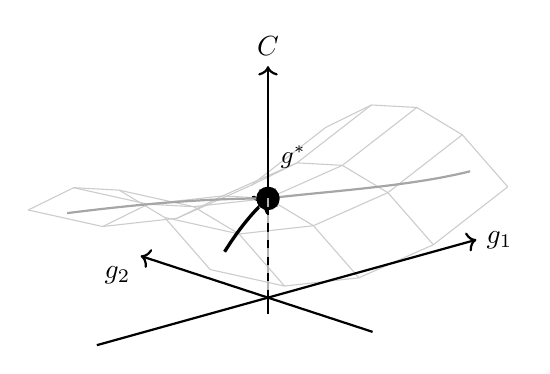
\begin{tikzpicture}[scale=1.05,
  x={({0.9cm,0.25cm})},
  y={({0cm,1cm})},
  z={({-0.55cm,0.18cm})}]
% Mesh of curved theory-space manifold (a saddle surface)
% z(x,z) = 0.15*(x-2)^2 - 0.15*(z-2)^2 + 1.2
\foreach \xi in {0,...,4} {
  \draw[gray!40,thin]
    (\xi,{0.15*(\xi-2)*(\xi-2)-0.15*(0-2)*(0-2)+1.2},0) --
    (\xi,{0.15*(\xi-2)*(\xi-2)-0.15*(1-2)*(1-2)+1.2},1) --
    (\xi,{0.15*(\xi-2)*(\xi-2)-0.15*(2-2)*(2-2)+1.2},2) --
    (\xi,{0.15*(\xi-2)*(\xi-2)-0.15*(3-2)*(3-2)+1.2},3) --
    (\xi,{0.15*(\xi-2)*(\xi-2)-0.15*(4-2)*(4-2)+1.2},4);
}
\foreach \zi in {0,...,4} {
  \draw[gray!40,thin]
    (0,{0.15*(0-2)*(0-2)-0.15*(\zi-2)*(\zi-2)+1.2},\zi) --
    (1,{0.15*(1-2)*(1-2)-0.15*(\zi-2)*(\zi-2)+1.2},\zi) --
    (2,{0.15*(2-2)*(2-2)-0.15*(\zi-2)*(\zi-2)+1.2},\zi) --
    (3,{0.15*(3-2)*(3-2)-0.15*(\zi-2)*(\zi-2)+1.2},\zi) --
    (4,{0.15*(4-2)*(4-2)-0.15*(\zi-2)*(\zi-2)+1.2},\zi);
}
% Axes in coupling-constant space
\draw[->,thick] (-0.3,0,2) -- (4.8,0,2) node[right] {$g_1$};
\draw[->,thick] (2,0,-0.3) -- (2,0,4.8) node[below left] {$g_2$};
\draw[->,thick] (2,-0.2,2) -- (2,2.8,2) node[above] {$C$};
% RG flow trajectories on the surface
\draw[->,very thick]
  (0.5,{0.15*(0.5-2)*(0.5-2)-0.15*(0.5-2)*(0.5-2)+1.2},0.5)
  ..controls (1,{0.15*(0.8-2)*(0.8-2)-0.15*(1-2)*(1-2)+1.2},1)
         and (1.5,{0.15*(1.2-2)*(1.2-2)-0.15*(1.5-2)*(1.5-2)+1.2},1.5)..
  (2,{0.15*(2-2)*(2-2)-0.15*(2-2)*(2-2)+1.2},2);
\draw[->,thick,gray!70]
  (3.8,{0.15*(3.8-2)*(3.8-2)-0.15*(0.5-2)*(0.5-2)+1.2},0.5)
  ..controls (3.3,{0.15*(3-2)*(3-2)-0.15*(1-2)*(1-2)+1.2},1)
         and (2.6,{0.15*(2.3-2)*(2.3-2)-0.15*(1.6-2)*(1.6-2)+1.2},1.7)..
  (2,{0.15*(2-2)*(2-2)-0.15*(2-2)*(2-2)+1.2},2);
\draw[->,thick,gray!70]
  (0.4,{0.15*(0.4-2)*(0.4-2)-0.15*(3.8-2)*(3.8-2)+1.2},3.8)
  ..controls (1,{0.15*(0.9-2)*(0.9-2)-0.15*(3.2-2)*(3.2-2)+1.2},3.2)
         and (1.5,{0.15*(1.4-2)*(1.4-2)-0.15*(2.5-2)*(2.5-2)+1.2},2.6)..
  (2,1.2,2);
% Fixed point
\node[circle,fill,inner sep=3pt] at (2,1.2,2) {};
\node[font=\small,above right] at (2.1,1.4,2.1) {$g^\ast$};
% Drop lines to base
\draw[dashed,gray!60] (2,1.2,2) -- (2,0,2);
\end{tikzpicture}
\caption{Renormalization group trajectories on a curved theory-space
manifold. The vertical coordinate is the monotonic $c$-function $C(g)$.
Multiple trajectories from different UV starting points flow downward
on this surface, converging toward the scale-invariant fixed point
$g^\ast$ at the minimum.}
\end{figure}

\section{Gradient Flows and Irreversibility}

Several results indicate that renormalization group flow behaves like a
gradient flow with respect to certain monotonic quantities
\cite{Zamolodchikov1986,Cardy1996}. In two dimensions, the $c$-theorem
establishes the existence of a function that decreases along RG
trajectories. More generally, RG evolution may be written as
\begin{equation}
\frac{d g^i}{d\tau} = -G^{ij} \frac{\partial C}{\partial g^j},
\end{equation}
where $C$ is a monotonic functional and $G^{ij}$ is a metric on theory
space. This structure resembles thermodynamic evolution, in which
systems move toward states of reduced free energy.

\begin{figure}[H]
\centering
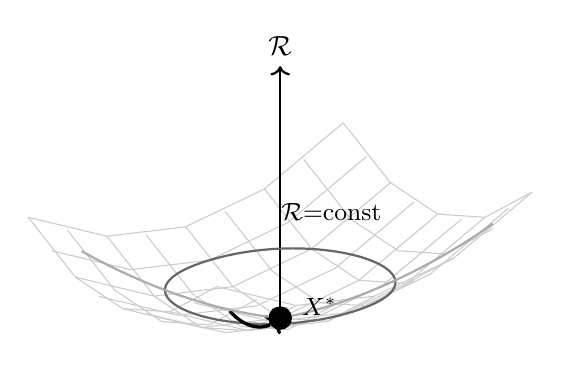
\begin{tikzpicture}[scale=1.0,
  x={({1.0cm,0.3cm})},
  y={({0cm,1cm})},
  z={({-0.6cm,0.22cm})}]
% A paraboloid bowl: y = 0.18*(x-2)^2 + 0.18*(z-2)^2
% Draw meridian curves
\foreach \xi in {0,0.5,...,4} {
  \draw[gray!40,thin]
    (\xi,{0.18*(\xi-2)*(\xi-2)+0.18*(0-2)*(0-2)},0) --
    (\xi,{0.18*(\xi-2)*(\xi-2)+0.18*(1-2)*(1-2)},1) --
    (\xi,{0.18*(\xi-2)*(\xi-2)+0.18*(2-2)*(2-2)},2) --
    (\xi,{0.18*(\xi-2)*(\xi-2)+0.18*(3-2)*(3-2)},3) --
    (\xi,{0.18*(\xi-2)*(\xi-2)+0.18*(4-2)*(4-2)},4);
}
\foreach \zi in {0,0.5,...,4} {
  \draw[gray!40,thin]
    (0,{0.18*(0-2)*(0-2)+0.18*(\zi-2)*(\zi-2)},\zi) --
    (1,{0.18*(1-2)*(1-2)+0.18*(\zi-2)*(\zi-2)},\zi) --
    (2,{0.18*(2-2)*(2-2)+0.18*(\zi-2)*(\zi-2)},\zi) --
    (3,{0.18*(3-2)*(3-2)+0.18*(\zi-2)*(\zi-2)},\zi) --
    (4,{0.18*(4-2)*(4-2)+0.18*(\zi-2)*(\zi-2)},\zi);
}
% Vertical axis
\draw[->,thick] (2,-0.1,2) -- (2,3.2,2) node[above] {$\mathcal{R}$};
% Level contour ring at height 1.0 (r^2 = 1/0.18 => r~2.36 too large; use r=1.5, y=0.18*1.5^2=0.405)
\draw[thick,black!60]
  (2,0.405,0.5) ..controls (3.5,0.405,0.5) and (3.5,0.405,3.5)..
  (2,0.405,3.5) ..controls (0.5,0.405,3.5) and (0.5,0.405,0.5)..
  (2,0.405,0.5);
% Descent trajectories
\draw[->,very thick]
  (0.4,{0.18*(0.4-2)*(0.4-2)+0.18*(0.4-2)*(0.4-2)},0.4)
  ..controls (0.9,{0.18*(0.9-2)*(0.9-2)+0.18*(0.9-2)*(0.9-2)},0.9)
         and (1.5,{0.18*(1.5-2)*(1.5-2)+0.18*(1.5-2)*(1.5-2)},1.5)..
  (2,0,2);
\draw[->,thick,gray!65]
  (3.8,{0.18*(3.8-2)*(3.8-2)+0.18*(0.5-2)*(0.5-2)},0.5)
  ..controls (3.3,{0.18*(3.3-2)*(3.3-2)+0.18*(0.9-2)*(0.9-2)},0.9)
         and (2.6,{0.18*(2.6-2)*(2.6-2)+0.18*(1.4-2)*(1.4-2)},1.4)..
  (2,0,2);
\draw[->,thick,gray!65]
  (0.5,{0.18*(0.5-2)*(0.5-2)+0.18*(3.7-2)*(3.7-2)},3.7)
  ..controls (1.0,{0.18*(1-2)*(1-2)+0.18*(3.2-2)*(3.2-2)},3.2)
         and (1.5,{0.18*(1.5-2)*(1.5-2)+0.18*(2.6-2)*(2.6-2)},2.6)..
  (2,0,2);
% Minimum
\node[circle,fill,inner sep=3pt] at (2,0,2) {};
\node[font=\small,right] at (2.15,0.1,2) {$X^\ast$};
% Label level contour
\node[font=\small] at (3.55,0.55,3.5) {$\mathcal{R}{=}\mathrm{const}$};
\end{tikzpicture}
\caption{Gradient flow on the entropy--coherence functional $\mathcal{R}$.
The paraboloid surface represents $\mathcal{R}$ over plenum field space.
Three descent trajectories from different initial conditions converge to
the minimum $X^\ast$, which corresponds to a stationary plenum regime.
Level sets of $\mathcal{R}$ are shown as closed curves on the bowl.}
\end{figure}

\section{The RSVP Plenum Framework}

The RSVP framework proposes that the universe can be described as a
continuous plenum governed by three interacting fields: a scalar density
field $\Phi$, a vector flow field $\mathbf{v}$, and an entropy field
$S$. Rather than treating spacetime curvature as fundamental, RSVP
interprets geometry as an emergent description of the organization of
these fields.

The dynamical evolution of the plenum can be expressed schematically as
\begin{align}
\partial_t \Phi &= F_\Phi(\Phi,\mathbf{v},S), \\
\partial_t \mathbf{v} &= F_v(\Phi,\mathbf{v},S), \\
\partial_t S &= F_S(\Phi,\mathbf{v},S).
\end{align}
These equations describe redistribution processes within the plenum.

\section{RSVP as a Geometric Flow}

A useful mathematical interpretation is to treat RSVP dynamics as a
gradient flow on a functional $\mathcal{R}$ defined over field space.
Let $X^A = (\Phi, \mathbf{v}, S)$ denote the collective fields. Then
the dynamics may be written as
\begin{equation}
\partial_t X^A = -G^{AB}\frac{\delta \mathcal{R}}{\delta X^B}.
\end{equation}
This formulation places RSVP within the broader family of geometric
flows that includes renormalization group evolution, Ricci flow
\cite{Hamilton1982}, and thermodynamic relaxation processes.

\begin{figure}[H]
\centering
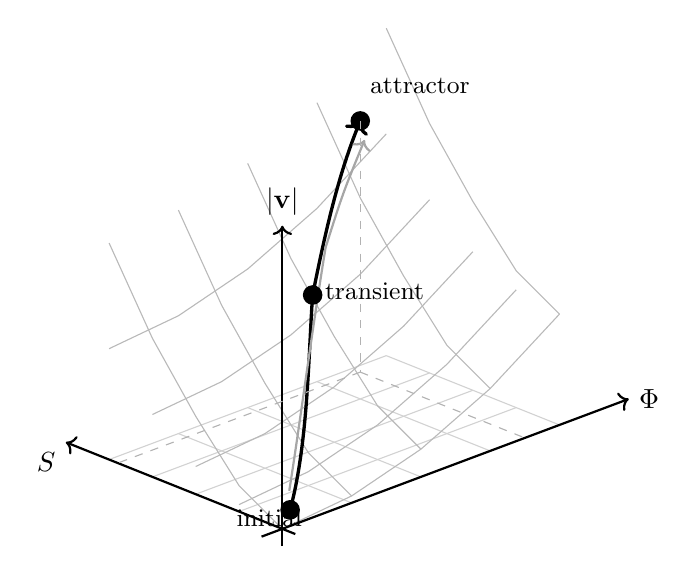
\begin{tikzpicture}[scale=1.1,
  x={({0.8cm,0.3cm})},
  y={({0cm,1cm})},
  z={({-0.5cm,0.2cm})}]
% Grid lines on base plane (y=0), representing S-Phi plane
\foreach \xi in {0,1,2,3,4} {
  \draw[gray!35,thin] (\xi,0,0) -- (\xi,0,4);
}
\foreach \zi in {0,1,2,3,4} {
  \draw[gray!35,thin] (0,0,\zi) -- (4,0,\zi);
}
% Curved surface: a saddle-like manifold lifted above base plane
% Parametric surface approximated by mesh curves
\foreach \xi in {0,1,2,3,4} {
  \draw[gray!55,thin]
    (\xi,{0.08*\xi*\xi},0) --
    (\xi,{0.08*\xi*\xi+0.3},1) --
    (\xi,{0.08*\xi*\xi+0.9},2) --
    (\xi,{0.08*\xi*\xi+1.6},3) --
    (\xi,{0.08*\xi*\xi+2.5},4);
}
\foreach \zi in {0,1,2,3,4} {
  \draw[gray!55,thin]
    (0,{0.08*\zi*\zi+0},\zi) --
    (1,{0.08*\zi*\zi+0.08},\zi) --
    (2,{0.08*\zi*\zi+0.32},\zi) --
    (3,{0.08*\zi*\zi+0.72},\zi) --
    (4,{0.08*\zi*\zi+1.28},\zi);
}
% Axes
\draw[->, thick] (-0.3,0,0) -- (5,0,0) node[right] {$\Phi$};
\draw[->, thick] (0,-0.2,0) -- (0,3.5,0) node[above] {$|\mathbf{v}|$};
\draw[->, thick] (0,0,-0.3) -- (0,0,5) node[below left] {$S$};
% Evolution trajectory on surface
\draw[->,very thick,black]
  (0.3,0.07,0.3) ..controls (1,0.5,1) and (1.5,1.2,1.8)..
  (2,1.6,2.5) ..controls (2.5,2.1,3) and (3,2.5,3.5)..
  (3.5,2.9,3.8);
% A second nearby trajectory
\draw[->,thick,gray!70]
  (0.6,0.1,0.8) ..controls (1.2,0.6,1.5) and (1.8,1.3,2.2)..
  (2.5,1.9,3.0) ..controls (3.0,2.3,3.4)..
  (3.5,2.7,3.7);
% Marked states
\node[circle,fill,inner sep=2.5pt] at (0.3,0.07,0.3) {};
\node[circle,fill,inner sep=2.5pt] at (2,1.6,2.5) {};
\node[circle,fill,inner sep=2.5pt] at (3.5,2.9,3.8) {};
\node[font=\small] at (0,0.07,0.3) {initial};
\node[font=\small,right] at (2.1,1.6,2.6) {transient};
\node[font=\small,above right] at (3.5,3.1,3.8) {attractor};
% Vertical dashed drop-lines from attractor to base
\draw[dashed,gray!60] (3.5,2.9,3.8) -- (3.5,0,3.8);
\draw[dashed,gray!60] (3.5,0,3.8) -- (3.5,0,0);
\draw[dashed,gray!60] (3.5,0,3.8) -- (0,0,3.8);
\end{tikzpicture}
\caption{Three-dimensional RSVP configuration manifold with coordinates
$(\Phi,|\mathbf{v}|,S)$. The manifold curves upward, reflecting
increasing coherence. The bold trajectory represents entropy-driven
evolution from an initial nonequilibrium state toward a coherent
attractor regime; the lighter trajectory shows a neighboring orbit
converging to the same attractor.}
\end{figure}

\section{Construction Principles for the RSVP Action}
\label{sec:principles}

The form of the RSVP action is constrained by several physical and
structural requirements, which we state explicitly before writing it
down. This prevents the Lagrangian from appearing as an arbitrary
ansatz.

\emph{Locality} requires that the Lagrangian density depend only on
the fields and their first derivatives at a point. This excludes
nonlocal integral kernels at leading order.

\emph{Rotational and translational invariance} restrict the allowed
scalar combinations of fields. In particular, the vector sector must
appear through scalars such as $\mathbf{v}^2$, $(\nabla \times
\mathbf{v})^2$, and $\mathbf{v} \cdot \nabla \Phi$.

\emph{Minimal coupling between sectors} requires that interaction
terms couple density, flow, and entropy at the lowest order consistent
with the symmetries, yielding three distinct coupling constants
$\lambda_1$, $\lambda_2$, $\lambda_3$ rather than a single universal
coupling.

\emph{Entropy production positivity} requires that the entropy balance
equation derived from the action admits a non-negative source term
$\sigma \geq 0$, consistent with the second law of thermodynamics.

\emph{Vorticity suppression} is motivated by the requirement that
small-scale turbulent flow be energetically penalized relative to
large-scale coherent structures. This is encoded by the term
$\kappa(\nabla \times \mathbf{v})^2$.

These five requirements uniquely determine the minimal action
functional up to the choice of potentials $V(\Phi)$ and $U(S)$ and the
values of the coupling constants.

\section{A Candidate RSVP Action Functional}
\label{sec:action}

To place the RSVP framework in closer analogy with conventional field
theory, we introduce an action functional governing the dynamics of the
plenum fields \cite{LandauFluid,MisnerThorneWheeler}. Let the
fundamental variables be $\Phi(x,t)$, $\mathbf{v}(x,t)$, and $S(x,t)$.

A minimal action functional may be written as
\begin{equation}
\mathcal{A}_{RSVP} =
\int d^4x \left[
\mathcal{L}_\Phi + \mathcal{L}_v + \mathcal{L}_S + \mathcal{L}_{\text{int}}
\right],
\end{equation}
with sector Lagrangians
\begin{align}
\mathcal{L}_\Phi &=
\frac{1}{2}(\partial_\mu \Phi)(\partial^\mu \Phi) - V(\Phi), \\
\mathcal{L}_v &=
\frac{1}{2}\rho(\Phi)\,\mathbf{v}^2 - \kappa(\nabla \times \mathbf{v})^2, \\
\mathcal{L}_S &=
\frac{1}{2}\alpha(\nabla S)^2 - U(S),
\end{align}
and interaction terms
\begin{equation}
\mathcal{L}_{\text{int}} =
\lambda_1 S\,\nabla \cdot \mathbf{v}
+ \lambda_2 \Phi S
+ \lambda_3 \mathbf{v} \cdot \nabla \Phi.
\end{equation}

\section{Variational Derivation of the RSVP Field Equations}

The dynamical equations follow from the Euler--Lagrange equations
\begin{equation}
\frac{\partial \mathcal{L}}{\partial \psi}
- \partial_\mu
\left(\frac{\partial \mathcal{L}}{\partial(\partial_\mu \psi)}\right) = 0
\end{equation}
applied to each field $\psi \in \{\Phi, \mathbf{v}, S\}$.

\subsection{Scalar Density Field}

For the scalar sector with interaction sourcing, the Euler--Lagrange
equation gives
\begin{equation}
\partial_\mu \partial^\mu \Phi + \frac{dV}{d\Phi} = J_\Phi,
\end{equation}
where the source term arising from the interaction Lagrangian is
\begin{equation}
J_\Phi = -\lambda_2 S - \lambda_3 \nabla \cdot \mathbf{v}
- \frac{1}{2}\frac{d\rho}{d\Phi}\,\mathbf{v}^2.
\end{equation}
This is a wave equation with a potential modified by entropy and flow
couplings.

\subsection{Vector Flow Field}

The vector sector yields an evolution equation resembling a generalized
forced Euler equation,
\begin{equation}
\rho(\Phi)\,\partial_t \mathbf{v} =
-\nabla P_{\text{eff}}
+ \kappa\,\nabla^2 \mathbf{v}
+ \mathbf{J}_v,
\end{equation}
where the effective pressure is
\begin{equation}
P_{\text{eff}} = \lambda_3 \Phi + \lambda_1 S,
\end{equation}
and the source $\mathbf{J}_v = \lambda_1 \nabla S + \lambda_3 \nabla \Phi$
arises from coupling gradients. The term $\kappa\,\nabla^2\mathbf{v}$
suppresses vorticity growth.

\subsection{Entropy Field}

For the entropy sector, variation yields
\begin{equation}
\alpha\,\nabla^2 S - \frac{dU}{dS} = J_S,
\end{equation}
with entropy source
\begin{equation}
J_S = -\lambda_1 \nabla \cdot \mathbf{v} - \lambda_2 \Phi.
\end{equation}
Together these three equations define the coupled dynamical system
governing RSVP plenum evolution.

\section{Explicit Form of the Entropy--Coherence Functional}
\label{sec:Rfunctional}

The gradient-flow formulation of RSVP requires a concrete
entropy--coherence functional $\mathcal{R}$ whose variation generates
the effective field evolution. We now construct it explicitly, unifying
the conservative action description with the dissipative gradient-flow
picture.

Motivated by the RSVP action and the requirement of monotonic entropy
production, we define
\begin{equation}
\mathcal{R}[\Phi,\mathbf{v},S] =
\int d^3x \Bigl[
\tfrac{1}{2}|\nabla \Phi|^2
+ \tfrac{1}{2}\rho(\Phi)|\mathbf{v}|^2
+ \tfrac{1}{2}\alpha|\nabla S|^2
+ V(\Phi) + U(S)
- \lambda_1 S\,\nabla \cdot \mathbf{v}
- \lambda_2 \Phi S
\Bigr].
\end{equation}
This functional combines energetic contributions (gradient and
potential terms) with entropy-flow couplings that encode
irreversibility and inter-field interaction.

\subsection{Functional Derivatives}

The functional derivatives of $\mathcal{R}$ with respect to the
fields are:
\begin{align}
\frac{\delta \mathcal{R}}{\delta \Phi} &=
-\nabla^2 \Phi + \frac{dV}{d\Phi}
- \lambda_2 S
+ \frac{1}{2}\frac{d\rho}{d\Phi}|\mathbf{v}|^2, \\
\frac{\delta \mathcal{R}}{\delta \mathbf{v}} &=
\rho(\Phi)\,\mathbf{v} + \lambda_1 \nabla S, \\
\frac{\delta \mathcal{R}}{\delta S} &=
-\alpha\,\nabla^2 S + \frac{dU}{dS}
- \lambda_1 \nabla \cdot \mathbf{v}
- \lambda_2 \Phi.
\end{align}

\subsection{Gradient Flow Dynamics}

With positive definite metric $G^{AB}$, the gradient-flow dynamics
\begin{equation}
\partial_t X^A = -G^{AB}\frac{\delta \mathcal{R}}{\delta X^B}
\end{equation}
yield
\begin{align}
\partial_t \Phi &= \nabla^2 \Phi - \frac{dV}{d\Phi}
+ \lambda_2 S
- \frac{1}{2}\frac{d\rho}{d\Phi}|\mathbf{v}|^2, \\
\partial_t \mathbf{v} &= -\rho(\Phi)\,\mathbf{v} - \lambda_1 \nabla S, \\
\partial_t S &= \alpha\,\nabla^2 S - \frac{dU}{dS}
+ \lambda_1 \nabla \cdot \mathbf{v} + \lambda_2 \Phi.
\end{align}
These equations reproduce, to leading order, the structure of the RSVP
field equations derived from the action functional, with the difference
that they describe dissipative relaxation toward entropy-coherent
configurations.

By Theorem~\ref{thm:gradient}, $\mathcal{R}$ is non-increasing along
trajectories,
\begin{equation}
\frac{d\mathcal{R}}{dt} \leq 0,
\end{equation}
with equality only at stationary points. Thus $\mathcal{R}$ serves as
a Lyapunov functional for RSVP dynamics.

\begin{remark}
The RSVP framework admits both a conservative formulation derived from
the action functional and a dissipative formulation generated by
$\mathcal{R}$. The latter may be viewed as an effective description
obtained after coarse-graining over microscopic degrees of freedom,
analogous to the emergence of thermodynamic behavior from underlying
Hamiltonian dynamics. The action description is the reversible backbone;
the gradient-flow description is its irreversible coarse-grained
shadow.
\end{remark}

\section{Conservation Laws}

The RSVP action possesses continuous symmetries that lead to
conservation laws through Noether's theorem \cite{Frankel,Nakahara}.

\subsection{Energy Functional}

The energy density associated with the plenum fields is
\begin{equation}
\mathcal{E} =
\frac{1}{2}|\partial_t\Phi|^2
+ \frac{1}{2}|\nabla \Phi|^2
+ \frac{1}{2}\rho(\Phi)|\mathbf{v}|^2
+ \kappa|\nabla \times \mathbf{v}|^2
+ \frac{1}{2}\alpha|\nabla S|^2
+ V(\Phi) + U(S).
\end{equation}
Under appropriate boundary conditions the total energy
\begin{equation}
E = \int \mathcal{E}\, d^3x
\end{equation}
is conserved. In the gradient-flow regime the energy decreases
monotonically, consistent with entropy-driven relaxation.

\subsection{Entropy Transport}

Entropy satisfies an advection--diffusion equation of the form
\begin{equation}
\partial_t S + \nabla \cdot (S\,\mathbf{v}) =
D_S\,\nabla^2 S + \sigma,
\end{equation}
where $D_S$ is the entropy diffusion coefficient and $\sigma \geq 0$
represents local entropy production. Integration over space gives
\begin{equation}
\frac{d}{dt}\int S\,d^3x = \int \sigma\,d^3x \geq 0,
\end{equation}
so total entropy is non-decreasing, consistent with the second law of
thermodynamics.

\section{Linear Stability Analysis}

To understand the formation of large-scale structure in RSVP dynamics,
consider small perturbations around a homogeneous equilibrium state
\cite{LandauFluid},
\begin{equation}
\Phi = \Phi_0 + \delta\Phi, \quad
\mathbf{v} = \delta\mathbf{v}, \quad
S = S_0 + \delta S.
\end{equation}
Linearizing the field equations around this background yields
\begin{align}
\partial_t \delta\Phi &=
D_\Phi\,\nabla^2 \delta\Phi + \lambda_2\,\delta S
+ \lambda_3\,\nabla \cdot \delta\mathbf{v}, \\
\partial_t \delta\mathbf{v} &=
-\frac{1}{\rho_0}\nabla\delta P_{\text{eff}}
+ \nu\,\nabla^2 \delta\mathbf{v}, \\
\partial_t \delta S &=
D_S\,\nabla^2 \delta S + \lambda_1\,\nabla \cdot \delta\mathbf{v}
+ \lambda_2\,\delta\Phi,
\end{align}
where $\nu = \kappa/\rho_0$ is an effective kinematic viscosity.

Assuming plane-wave solutions $\delta X \propto e^{i(\mathbf{k}\cdot\mathbf{x} - \omega t)}$,
one obtains the dispersion relation for longitudinal modes,
\begin{equation}
\omega^2 = \left(D_\Phi + D_S - \frac{\lambda_1\lambda_3}{\rho_0}\right)k^2
- \lambda_2^2 + \mathcal{O}(k^4).
\end{equation}
Instabilities occur when the effective sound-speed term becomes
negative. In particular, when the coupling $\lambda_2^2$ between density
and entropy fields exceeds the diffusive stabilization, long-wavelength
modes become unstable, which provides a mechanism for spontaneous
formation of large-scale coherent structures.

\section{Spectral Representation of RSVP Fields}

The plenum fields can be expanded in Fourier modes,
\begin{equation}
\Phi(x,t) = \int \tilde{\Phi}(k,t)\, e^{ik \cdot x}\, d^3k,
\end{equation}
and similarly for $\mathbf{v}$ and $S$. In this representation
coarse-graining corresponds to removing high-frequency modes $|k| > \Lambda$.
The resulting effective fields obey renormalized dynamical equations
in which coupling parameters depend on the cutoff scale $\Lambda$.
This provides a direct connection between RSVP field evolution and
renormalization group methods \cite{Wilson1974,Polchinski1984}.

\section{Continuum Limit of Spherepop Dynamics}
\label{sec:continuumlimit}

We now formalize the relationship between the discrete Spherepop event
structure of Section~\ref{sec:spherepop} and the continuous RSVP field
description.

\subsection{Assumptions on the Event Ensemble}

We assume that the Spherepop event configuration $\{e_i\}$ satisfies:
\begin{enumerate}
\item \emph{Locality}: each event affects only a bounded neighborhood,
\item \emph{Finite propagation}: interactions propagate at finite speed,
\item \emph{Statistical regularity}: event distributions admit
coarse-grained averages over sufficiently large regions.
\end{enumerate}

\begin{theorem}[Emergence of RSVP Field Dynamics]
\label{thm:reduction}
Consider a sequence of Spherepop event configurations with
coarse-graining scale $\ell \to 0$ and event density increasing such
that macroscopic observables remain finite. Under the assumptions of
locality, finite propagation speed, and statistical regularity, the
coarse-grained fields $(\Phi_\ell, \mathbf{v}_\ell, S_\ell)$ converge
weakly to continuous fields $(\Phi, \mathbf{v}, S)$ satisfying a system
of coupled partial differential equations
\begin{equation}
\partial_t X^A = F^A(X,\nabla X).
\end{equation}
Moreover, if the microscopic event dynamics conserve total density
and respect entropy production constraints, the limiting equations
take the form of a gradient flow
\begin{equation}
\partial_t X^A = -G^{AB}\frac{\delta \mathcal{R}}{\delta X^B}
\end{equation}
for a functional $\mathcal{R}$ determined by the coarse-grained
statistics of the event ensemble.
\end{theorem}

\begin{proof}[Sketch]
The proof follows standard arguments in hydrodynamic and kinetic limits.
Local averaging defines effective fields whose evolution is determined
by the net flux of conserved quantities across the boundary of
$B_\ell(x)$. Locality ensures that only nearby events contribute to
the flux, while finite propagation bounds the rate of change.
Statistical regularity guarantees convergence of empirical averages to
smooth fields as $\ell \to 0$.

Conservation of density produces a continuity equation; the
momentum-like transfer $\mathbf{j}(e_i)$ defines the effective flow
field $\mathbf{v}$. Entropy production at the microscopic level induces
a monotonic functional $\mathcal{R}$ whose variation governs relaxation.
Collecting these contributions yields a closed system for
$(\Phi,\mathbf{v},S)$, which can be written in gradient-flow form under
positivity conditions on the coarse-grained metric $G^{AB}$.
\end{proof}

\begin{remark}
The structure of Theorem~\ref{thm:reduction} closely parallels the
derivation of hydrodynamics from kinetic theory and the emergence of
effective field theories under renormalization group flow. In this sense,
RSVP dynamics may be interpreted as the hydrodynamic limit of an
underlying event-based theory.
\end{remark}

\section{Topological Structures in the Plenum}

The vector flow field $\mathbf{v}$ admits conserved topological
invariants \cite{ArnoldKhesin}.

\begin{definition}
The helicity of the plenum flow is
\begin{equation}
H = \int \mathbf{v} \cdot (\nabla \times \mathbf{v})\, d^3x.
\end{equation}
\end{definition}

Under the RSVP evolution equations with appropriate boundary conditions,
$H$ is conserved in the inviscid limit $\kappa \to 0$. Physically,
helicity measures the degree to which flow lines are linked and twisted.

The linking number of two closed vortex curves $\gamma_1$, $\gamma_2$
is given by the Gauss integral
\begin{equation}
L(\gamma_1,\gamma_2) =
\frac{1}{4\pi}
\oint_{\gamma_1}\oint_{\gamma_2}
\frac{(\mathbf{r}_1 - \mathbf{r}_2)
      \cdot (d\mathbf{r}_1 \times d\mathbf{r}_2)}
     {|\mathbf{r}_1 - \mathbf{r}_2|^3}.
\end{equation}
Vortex structures with nontrivial topology can trap entropy and density
gradients, providing a mechanism for the persistence of coherent
cosmic structures over long timescales.

\begin{figure}[H]
\centering
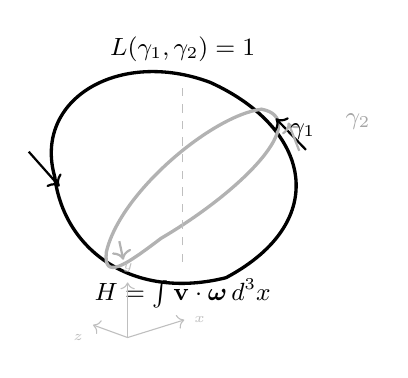
\begin{tikzpicture}[scale=1.0,
  x={({0.9cm,0.28cm})},
  y={({0cm,1cm})},
  z={({-0.55cm,0.2cm})}]
% Two linked torus-knot-style vortex tubes
% Tube 1: a loop in the xz-plane tilted slightly
% Approximate as ellipse projected
\draw[very thick,black]
  (2,0.0,1) ..controls (3.5,0.3,1) and (3.8,1.2,2)..
  (3,1.8,3) ..controls (2.2,2.3,3.8) and (0.8,2.1,3.5)..
  (0.5,1.4,2.5) ..controls (0.2,0.7,1.8) and (0.8,0.0,1.2)..
  (2,0.0,1);
% Tube 2: a loop in a perpendicular plane, linked with tube 1
\draw[very thick,gray!60]
  (2,0.2,2.5) ..controls (3.2,0.5,2.5) and (3.5,1.5,1.5)..
  (2.5,2.0,1.0) ..controls (1.5,2.3,0.5) and (0.5,1.5,1.0)..
  (0.8,0.5,1.8) ..controls (1.0,0.0,2.2) and (1.5,0.0,2.5)..
  (2,0.2,2.5);
% Flow arrows along tube 1
\draw[->,thick] (3.8,0.9,2.1) -- (3.65,1.25,2.55);
\draw[->,thick] (0.5,1.6,3.1) -- (0.75,1.15,2.8);
% Flow arrows along tube 2
\draw[->,thick,gray!60] (3.4,1.1,1.6) -- (3.0,1.65,1.2);
\draw[->,thick,gray!60] (0.8,0.7,1.5) -- (1.1,0.3,1.9);
% Vorticity labels
\node[font=\small] at (4.0,1.0,2.5) {$\gamma_1$};
\node[font=\small,gray!70] at (3.8,1.5,0.9) {$\gamma_2$};
% Linking number label
\node[font=\small] at (2,2.7,2) {$L(\gamma_1,\gamma_2)=1$};
% Helicity annotation
\draw[dashed,gray!50] (2,0,2) -- (2,2.3,2);
\node[font=\small] at (2,-0.4,2) {$H=\int\mathbf{v}\cdot\boldsymbol{\omega}\,d^3x$};
% Axes (small, in corner)
\draw[->,gray!50,thin] (0,0,0) -- (0.8,0,0) node[right,font=\tiny] {$x$};
\draw[->,gray!50,thin] (0,0,0) -- (0,0.7,0) node[above,font=\tiny] {$y$};
\draw[->,gray!50,thin] (0,0,0) -- (0,0,0.8) node[below left,font=\tiny] {$z$};
\end{tikzpicture}
\caption{Two linked vortex tubes $\gamma_1$ (black) and $\gamma_2$
(gray) in the plenum flow field $\mathbf{v}$. Their topological linking
number $L(\gamma_1,\gamma_2)=1$ is a conserved invariant in the inviscid
limit. The global helicity $H = \int\mathbf{v}\cdot(\nabla\times\mathbf{v})\,d^3x$
measures the total winding and is conserved under RSVP evolution when
$\kappa\to 0$. Such topological structures can trap entropy gradients,
stabilizing coherent cosmic configurations.}
\end{figure}

\section{Curvature of Theory Space and the Zamolodchikov Metric}

The geometric interpretation of renormalization group flow becomes more
precise when the space of couplings is endowed with a metric structure.
In two-dimensional conformal field theory, Zamolodchikov demonstrated
that the space of marginal couplings carries a natural Riemannian metric
defined by two-point functions of operators \cite{Zamolodchikov1986}.

Let $g_i$ denote couplings associated with operators $\mathcal{O}_i$.
The Zamolodchikov metric is
\begin{equation}
G_{ij} \sim \langle \mathcal{O}_i(x)\,\mathcal{O}_j(0)\rangle.
\end{equation}
Under RG flow, couplings evolve along geodesics of this curved
manifold. The curvature of theory space reflects operator mixing and
quantum corrections \cite{PannellStergiou2025}.

In RSVP theory, the universe evolves through a configuration space
defined by $(\Phi,\mathbf{v},S)$. If this space is endowed with an
appropriate metric $G^{AB}$, dynamical evolution corresponds to
trajectories in a curved field manifold. The geometric structure of
theory space in quantum field theory may therefore have a precise
analogue in the geometric structure of plenum field space.

\section{Entropy, Holography, and Emergent Geometry}

The connection between entropy and spacetime geometry has become a
central theme in modern theoretical physics
\cite{tHooft1993,Susskind1995,Maldacena1998}. Black hole thermodynamics
revealed that gravitational systems possess entropy proportional to
horizon area \cite{Bekenstein1973,Hawking1975}.

In the AdS/CFT correspondence, spacetime geometry in a bulk gravitational
theory emerges from the entanglement structure of a boundary quantum
field theory \cite{Maldacena1998,RyuTakayanagi2006,Swingle2012}. More
broadly, Ryu--Takayanagi formula relates entanglement entropy of a
boundary region to the area of a minimal bulk surface.

The RSVP framework offers a complementary interpretation. Instead of
deriving geometry from boundary entanglement, RSVP treats entropy as
one of the primary dynamical fields. The entropy field $S$ interacts
with density $\Phi$ and flow $\mathbf{v}$, producing large-scale
structures through redistribution processes. Geometric properties of
spacetime arise from the collective organization of these fields as
coherent patterns stabilize.

\begin{figure}[H]
\centering
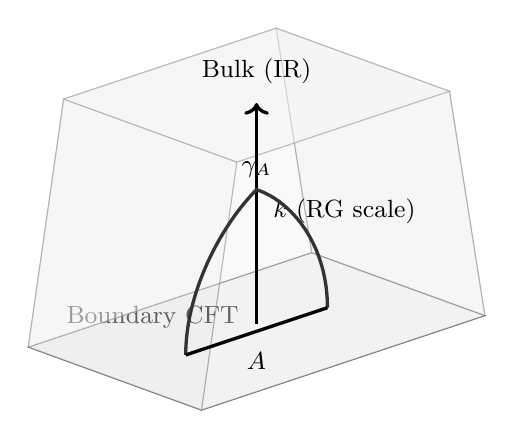
\begin{tikzpicture}[scale=1.0,
  x={({0.9cm,0.3cm})},
  y={({0cm,1cm})},
  z={({-0.55cm,0.2cm})}]
% AdS-like slab: boundary at y=0, bulk extends in y direction
% Boundary plane (y=0)
\draw[black!70,fill=gray!15,opacity=0.8]
  (0,0,0) -- (4,0,0) -- (4,0,4) -- (0,0,4) -- cycle;
\node[font=\small] at (2,-0.3,4.4) {Boundary CFT};
% Bulk region (wedge above boundary)
\draw[black!50,fill=gray!8,opacity=0.4]
  (0,0,0) -- (4,0,0) -- (3.5,3,0) -- (0.5,3,0) -- cycle;
\draw[black!50,fill=gray!8,opacity=0.4]
  (0,0,4) -- (4,0,4) -- (3.5,3,4) -- (0.5,3,4) -- cycle;
\draw[black!50,fill=gray!12,opacity=0.4]
  (0,0,0) -- (0,0,4) -- (0.5,3,4) -- (0.5,3,0) -- cycle;
\draw[black!50,fill=gray!12,opacity=0.4]
  (4,0,0) -- (4,0,4) -- (3.5,3,4) -- (3.5,3,0) -- cycle;
% Top of bulk (IR cutoff slice)
\draw[black!40,fill=gray!10,opacity=0.5]
  (0.5,3,0) -- (3.5,3,0) -- (3.5,3,4) -- (0.5,3,4) -- cycle;
\node[font=\small] at (2,3.3,2) {Bulk (IR)};
% Radial direction arrow
\draw[->,very thick] (2,0.1,2) -- (2,2.9,2);
\node[font=\small,right] at (2.1,1.5,2) {$k$ (RG scale)};
% Minimal surface (Ryu-Takayanagi) arc in bulk
\draw[very thick,black!80]
  (1,0,2) ..controls (1,0.8,2) and (1.5,1.5,2)..
  (2,1.8,2) ..controls (2.5,1.5,2) and (3,0.8,2)..
  (3,0,2);
\node[font=\small] at (2,2.05,2) {$\gamma_A$};
% Boundary interval
\draw[very thick] (1,0,2) -- (3,0,2);
\node[font=\small,below] at (2,-0.15,2) {$A$};
\end{tikzpicture}
\caption{Holographic geometry with boundary conformal field theory at
$y=0$ and bulk Anti-de Sitter spacetime above it. The radial coordinate
corresponds to the RG scale $k$. The arc $\gamma_A$ is the
Ryu--Takayanagi minimal surface in the bulk whose area computes the
entanglement entropy of boundary region $A$. In the RSVP interpretation,
the radial direction corresponds to entropy-driven smoothing across
plenum scales.}
\end{figure}

\section{RSVP Dynamics as Coarse-Grained Renormalization Flow}

The similarity between RSVP evolution and renormalization group flow
becomes clearer when coarse-graining procedures are considered.

In quantum field theory, coarse-graining integrates out short-distance
degrees of freedom, corresponding to
\begin{equation}
\Gamma_\Lambda[\phi] \rightarrow \Gamma_{\Lambda - d\Lambda}[\phi],
\end{equation}
where $\Lambda$ is a momentum cutoff. A conceptually similar process
occurs in RSVP dynamics. A coarse-graining transformation acts on the
plenum fields as
\begin{equation}
X^A(x) \rightarrow \bar{X}^A(x) = \int K(x-y)\,X^A(y)\,dy,
\end{equation}
where $K$ is a smoothing kernel. The evolution of the coarse-grained
fields defines a flow on the space of plenum configurations, analogous
to RG flow on theory space. Large-scale cosmological behavior
corresponds to infrared fixed points of the plenum evolution.

\section{Renormalization Flow Derived from the RSVP Action}

Following the functional renormalization group approach
\cite{Reuter1998,ZinnJustin}, the scale dependence of the effective
RSVP action can be expressed as
\begin{equation}
\partial_k \Gamma_k[\Phi,\mathbf{v},S] =
\frac{1}{2}
\mathrm{Tr}\left[
(\Gamma_k^{(2)} + R_k)^{-1}\partial_k R_k
\right],
\end{equation}
where $\Gamma_k^{(2)}$ denotes the second functional derivative and
$R_k$ is an infrared regulator. The effective action depends on all
three plenum fields, so the trace runs over $(\Phi,\mathbf{v},S)$
fluctuation modes. This equation describes how the effective
interactions among density, vector flow, and entropy fields evolve as
small-scale plenum fluctuations are integrated out, establishing a
direct mathematical bridge between conventional RG analysis and
entropy-driven plenum dynamics.

\section{Entropy Production and Irreversibility}

Irreversibility plays an important role in both thermodynamics and RG
dynamics \cite{Jaynes1957,Jaynes1957b,Callen}. Define the local entropy
production rate
\begin{equation}
\sigma = D_S|\nabla S|^2 / S + \kappa|\nabla \times \mathbf{v}|^2,
\end{equation}
which combines diffusive entropy production and viscous dissipation.
The entropy balance equation
\begin{equation}
\partial_t S + \nabla \cdot (S\,\mathbf{v}) = D_S\,\nabla^2 S + \sigma
\end{equation}
then describes both entropy transport and production simultaneously.
The positive definiteness of $\sigma$ ensures irreversibility,
providing a microscopic basis for the monotonic decrease of the
entropy--coherence functional $\mathcal{R}$ established in
Theorem~\ref{thm:gradient} below.

\section{Hamiltonian Formulation of RSVP Field Dynamics}

An equivalent formulation of RSVP dynamics uses canonical momenta
and Hamiltonian mechanics \cite{Frankel,Nakahara,BaezMunian}.

Define conjugate momenta
\begin{align}
\Pi_\Phi &= \frac{\partial \mathcal{L}}{\partial(\partial_t \Phi)}
= \partial_t \Phi, \\
\boldsymbol{\Pi}_v &= \frac{\partial \mathcal{L}}{\partial(\partial_t \mathbf{v})}
= \rho(\Phi)\,\mathbf{v}, \\
\Pi_S &= \frac{\partial \mathcal{L}}{\partial(\partial_t S)} = 0.
\end{align}
The Hamiltonian density is obtained by Legendre transform:
\begin{equation}
\mathcal{H} =
\frac{1}{2}\Pi_\Phi^2
+ \frac{|\boldsymbol{\Pi}_v|^2}{2\rho(\Phi)}
+ \frac{1}{2}|\nabla \Phi|^2
+ \frac{1}{2}\alpha|\nabla S|^2
+ \kappa|\nabla\times\mathbf{v}|^2
+ V(\Phi) + U(S)
+ \mathcal{H}_{\text{int}}.
\end{equation}
The Hamilton equations of motion
\begin{equation}
\partial_t X^A = \frac{\delta \mathcal{H}}{\delta \Pi_A}, \qquad
\partial_t \Pi_A = -\frac{\delta \mathcal{H}}{\delta X^A}
\end{equation}
reproduce the Euler--Lagrange equations derived in Section~9. The
configuration space of plenum fields becomes a phase space equipped
with the symplectic form
\begin{equation}
\Omega = \int d^3x\, d\Pi_A \wedge dX^A.
\end{equation}

\begin{remark}
The entropy field $S$ has vanishing canonical momentum at this order.
In an extended formulation incorporating entropy production explicitly,
a Lagrange multiplier for the entropy balance constraint introduces a
nontrivial conjugate variable representing a chemical potential.
\end{remark}

\section{Lie Symmetry Structure of Plenum Dynamics}

Continuous symmetries of the RSVP action generate conserved currents
via Noether's theorem \cite{Frankel,WeinbergQFT}. Under the
infinitesimal coordinate transformation $x^\mu \to x^\mu + \epsilon\xi^\mu$
together with field variations $\delta\Phi$, $\delta\mathbf{v}$,
$\delta S$, the action is invariant when
\begin{equation}
\delta\mathcal{A}_{RSVP} = 0.
\end{equation}

The generators of symmetry transformations form a Lie algebra
\begin{equation}
[T_a, T_b] = f_{ab}^{\;\;c}\,T_c,
\end{equation}
where $f_{ab}^{\;\;c}$ are the structure constants. The principal
symmetries of the RSVP action include spatial translation invariance,
generating momentum conservation in the plenum; rotational invariance,
generating angular momentum conservation for the vector flow field;
and global shifts $S \to S + \text{const}$, which are broken by the
potential $U(S)$ to a discrete subgroup. The study of these symmetries
classifies invariant solutions and attractor configurations within
RSVP dynamics.

\section{Lie Algebra Cascade of Entropy Flow}

Entropy transport in RSVP dynamics can be interpreted as a cascade of
transformations generated by vector flow operators. The entropy field
evolves according to
\begin{equation}
\partial_t S = \mathcal{L}_{\mathbf{v}} S + D_S\,\nabla^2 S + \sigma,
\end{equation}
where $\mathcal{L}_{\mathbf{v}}$ is the Lie derivative along the flow
field. Successive interactions between flow modes generate a cascade
analogous to a Lie algebra action on tensor fields. Letting $T_a$
denote generators associated with flow modes at scale $a$, the
algebra satisfies $[T_a, T_b] = f_{ab}^{\;\;c} T_c$. Entropy
redistribution across scales can therefore be interpreted as a sequence
of Lie algebra operations progressively transferring structure from
small to large scales.

\section{Correspondence Between RG and RSVP}

The structural similarities between RG flow and RSVP dynamics suggest
a precise correspondence. In both frameworks, microscopic complexity
is progressively reorganized into effective macroscopic behavior.

\medskip
\begin{center}
\begin{tabular}{@{} p{0.44\textwidth} p{0.44\textwidth} @{}}
\toprule
Renormalization Group & RSVP \\
\midrule
Theory space trajectory    & Plenum field trajectory \\
RG fixed point             & Stationary plenum regime \\
Coarse-graining            & Entropic smoothing \\
Monotonic $c$-function     & Entropy--coherence functional $\mathcal{R}$ \\
Zamolodchikov metric       & Field-space metric $G^{AB}$ \\
UV cutoff $\Lambda$        & Smoothing kernel scale \\
Operator mixing matrix     & Field coupling matrix $\lambda_{ij}$ \\
\bottomrule
\end{tabular}
\end{center}
\medskip

\begin{figure}[H]
\centering
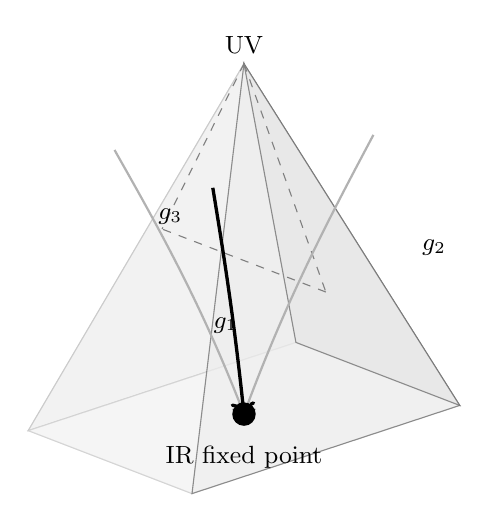
\begin{tikzpicture}[scale=1.0,
  x={({0.85cm,0.28cm})},
  y={({0cm,1cm})},
  z={({-0.52cm,0.2cm})}]
\coordinate (apex) at (2,4.5,2);
\coordinate (B1) at (0,0,0);
\coordinate (B2) at (4,0,0);
\coordinate (B3) at (4,0,4);
\coordinate (B4) at (0,0,4);
\draw[gray!50,fill=gray!10,opacity=0.6] (apex) -- (B1) -- (B4) -- cycle;
\draw[gray!50,fill=gray!12,opacity=0.6] (apex) -- (B4) -- (B3) -- cycle;
\draw[gray!40,fill=gray!8,opacity=0.5] (B1) -- (B2) -- (B3) -- (B4) -- cycle;
\draw[black!60,fill=gray!15,opacity=0.7] (apex) -- (B1) -- (B2) -- cycle;
\draw[black!60,fill=gray!20,opacity=0.7] (apex) -- (B2) -- (B3) -- cycle;
\coordinate (M1) at (2,2,0);
\coordinate (M2) at (2,2,4);
\draw[black!50,dashed] (apex) -- (M1);
\draw[black!50,dashed] (apex) -- (M2);
\draw[black!50,dashed] (M1) -- (M2);
\draw[->,very thick]
  (0.8,3.5,0.8) ..controls (1.2,2.5,1.2) and (1.6,1.5,1.6)..
  (2.0,0.05,2.0);
\draw[->,thick,gray!60]
  (3.2,3.5,0.8) ..controls (2.8,2.5,1.2) and (2.4,1.5,1.6)..
  (2.0,0.05,2.0);
\draw[->,thick,gray!60]
  (0.8,3.5,3.2) ..controls (1.2,2.5,2.8) and (1.6,1.5,2.4)..
  (2.0,0.05,2.0);
\node[circle,fill,inner sep=3pt] at (2,0.05,2) {};
\node[font=\small,above] at (apex) {UV};
\node[font=\small] at (2,-0.5,2) {IR fixed point};
\node[font=\small] at (0.5,2,0) {$g_1$};
\node[font=\small] at (3.8,2,0.3) {$g_2$};
\node[font=\small] at (2,2.2,3.8) {$g_3$};
\end{tikzpicture}
\caption{Theory space as a three-dimensional polyhedral cone. The apex
represents the ultraviolet regime; the three faces correspond to sectors
dominated by couplings $g_1$, $g_2$, $g_3$. Renormalization group
trajectories flow along the faces of the cone, converging to the
infrared fixed point at the base center.}
\end{figure}

\section{Related Work}
\label{sec:relatedwork}

A growing body of work in theoretical physics has explored the
possibility that geometry, gravitation, and physical law may arise from
informational, entropic, or emergent structures. Jacobson's thermodynamic
derivation of the Einstein equation showed that gravitational dynamics
can be interpreted as an equation of state associated with local horizon
thermodynamics \cite{Jacobson1995}. Verlinde extended this direction by
proposing that gravity may be understood as an entropic force
\cite{Verlinde2011}. Within holographic and entanglement-based
approaches, Ryu--Takayanagi and developments by Van Raamsdonk
strengthened the view that spacetime connectivity may be reconstructed
from entanglement structure \cite{RyuTakayanagi2006,VanRaamsdonk2010}.

In the study of renormalization and theory space, the irreversibility of
RG flow and the geometry of operator manifolds suggest that physical
description carries an intrinsic directional and geometric organization
\cite{Zamolodchikov1986,PannellStergiou2025}. Jaynes and Landauer each
contributed foundational perspectives connecting inference, entropy, and
physical law \cite{Jaynes1957,Landauer1961}.

The symbolic collapse grammar framework of Taylor belongs to this broad
lineage but approaches it from the side of discrete symbolic emergence
\cite{Taylor2025}. There, physical observables arise from motif
rendering, entropy-weighted collapse, and symbolic grammar over a binary
alphabet. The RSVP framework proposed here shares with such approaches
the conviction that physical structure is emergent and entropy-sensitive,
but differs in a decisive respect: rather than taking symbolic collapse
as primitive, RSVP posits continuous scalar, vector, and entropy fields
whose coupled dynamics generate both geometric structure and, in suitable
discrete limits, symbolic rendering rules. In this sense, RSVP is
intended not as a competitor to discrete emergence models but as a
possible field-theoretic completion within which they may be recovered as
coarse-grained projections.

\section{Symbolic Collapse Grammars as Discrete Limits of the Plenum}
\label{sec:symboliccollapse}

\subsection{Overview}

Symbolic collapse grammars model physical emergence as a
rendering process constrained by entropy. Motifs are evaluated by
an entropy cost functional; only those satisfying a threshold
condition are permitted to render as physical states.

We show here that such grammars are recovered as a discrete,
thresholded, overdamped limit of RSVP dynamics.

\subsection{Discrete Symbolic Substrate}

Let the symbolic alphabet be
\[
\Sigma = \{A,\, A^\perp\}.
\]
Define an embedding into the scalar field $\Phi(x,t)$ by
\[
A \mapsto +\phi_0, \qquad A^\perp \mapsto -\phi_0,
\]
for fixed amplitude $\phi_0 > 0$. A symbolic motif of length $N$,
\[
w = (s_1,\dots,s_N), \quad s_i \in \Sigma,
\]
corresponds to a discrete sampling of $\Phi$ over a lattice
$\{x_i\}_{i=1}^N$, so the symbolic substrate is equivalent to a
binary-valued lattice field configuration.

\subsection{Entropy Functional as Coarse-Grained Field}

The symbolic entropy cost $H(w)$ is identified with the coarse-grained
entropy field:
\[
H(w) \approx \sum_{i=1}^N S(x_i,t)
\;\longrightarrow\;
\int_\Omega S(x,t)\, dV.
\]
The symbolic entropy measure is therefore the discrete projection of a
continuous entropy density.

\subsection{Collapse Operator as Thresholded Dynamics}

The symbolic collapse rule
\[
\hat{M}(w) =
\begin{cases}
\text{rendered}, & H(w) < H_c, \\
\varnothing, & \text{otherwise}
\end{cases}
\]
is reproduced by the local collapse indicator
\[
\chi(x,t) = \Theta\big(S_c - S(x,t) - \alpha\,\nabla\cdot\mathbf{v}(x,t)\big),
\]
where $\Theta$ is the Heaviside function. The global symbolic condition
$H(w) < H_c$ is the integrated constraint $\int_\Omega S\,dV < H_c$,
which is an observable derived from field dynamics rather than a
primitive rule.

\subsection{Variational Embedding and the RSVP Lagrangian}

To make the discrete-limit argument variational, we record the full
RSVP Lagrangian density:
\begin{align}
\mathcal{L}_{RSVP} &=
\frac{1}{2}(\partial_t\Phi)^2 - \frac{c_\Phi^2}{2}|\nabla\Phi|^2
- U(\Phi) \notag \\
&\quad + \frac{\rho_v}{2}|\partial_t\mathbf{v}|^2
- \frac{\nu_v^2}{2}|\nabla\mathbf{v}|^2
- \frac{m_v^2}{2}|\mathbf{v}|^2 \notag \\
&\quad + \frac{\rho_S}{2}(\partial_t S)^2
- \frac{c_S^2}{2}|\nabla S|^2 - W(S) \notag \\
&\quad + \kappa\,S\Phi + \alpha\,\mathbf{v}\cdot\nabla\Phi
+ \beta\,\mathbf{v}\cdot\nabla S
- \gamma\,S\,\nabla\cdot\mathbf{v}
- \delta\,\Phi^2 S,
\end{align}
with quartic potentials $U(\Phi) = \tfrac{\lambda}{4}\Phi^4 -
\tfrac{\mu_\Phi^2}{2}\Phi^2$ and $W(S) = \tfrac{\lambda_S}{4}S^4 -
\tfrac{\mu_S^2}{2}S^2$. Adding a Rayleigh dissipation functional
\[
\mathcal{R}_{dis} = \int\left(
\tfrac{\sigma_\Phi}{2}(\partial_t\Phi)^2
+ \tfrac{\sigma_v}{2}|\partial_t\mathbf{v}|^2
+ \tfrac{\sigma_S}{2}(\partial_t S)^2
\right)d^nx
\]
and passing to the overdamped limit $\sigma\to\infty$ reduces the
second-order system to a first-order gradient flow, recovering the
effective RSVP evolution equations.

\subsection{Reduction Theorem}

\begin{theorem}[Overdamped Binary Reduction]
\label{thm:symbolicreduction}
Consider the RSVP Lagrangian above with Rayleigh dissipation. In the
simultaneous limits
\begin{alignat*}{2}
&\textup{(i)}\quad && \sigma_\Phi,\sigma_v,\sigma_S \to \infty
  \quad\textup{(overdamped)}, \\
&\textup{(ii)}\quad && \Phi(x,t)\in\{+\phi_0,-\phi_0\}
  \quad\textup{(binary scalar)}, \\
&\textup{(iii)}\quad && \mathbf{v}(x,t)\to 0
  \quad\textup{(suppressed flow)}, \\
&\textup{(iv)}\quad && S(x,t)\to S_i\;\textup{piecewise constant},
  \quad\partial_t(\Phi,S)\to 0
  \quad\textup{(quasi-static)},
\end{alignat*}
the RSVP system reduces to a symbolic collapse grammar over
$\Sigma=\{A,A^\perp\}$ with rendering rule determined by a
thresholded entropy functional.
\end{theorem}

\begin{proof}
In the overdamped limit, inertial terms vanish and the Euler--Lagrange
equations reduce to gradient-flow form
\[
\sigma_q\,\partial_t q \approx -\frac{\delta L}{\delta q},
\]
so the system evolves toward local minima of the effective energy
functional $E[\Phi,\mathbf{v},S]$.

Under the binary constraint on $\Phi$, the field reduces to a
discrete-valued function on a partition $\{\Omega_i\}$, identified with
a symbolic string $w$. Since $\mathbf{v}\to 0$, all transport and
flow-coupling terms vanish. The entropy field becomes piecewise
constant, so the total entropy reduces to the finite sum
$H(w) = \sum_i S_i|\Omega_i|$.

The RSVP collapse indicator reduces to the global condition
$\sum_i S_i < H_c$, which reproduces the symbolic collapse rule.
\end{proof}

\begin{corollary}[Loss of Geometric Information]
The reduction to symbolic collapse dynamics eliminates entropy
gradients $\nabla S$, vector flow $\mathbf{v}$, and continuous scalar
variation. Any metric of the form $g_{ij} \sim \partial_i S\partial_j S
+ v_iv_j + \Phi^2\delta_{ij}$ reduces to a trivial or piecewise
constant structure. Therefore symbolic grammars constitute a strictly
lower-dimensional representation of plenum dynamics: they are
projections, not equivalents.
\end{corollary}

\begin{remark}
The relationship between RSVP and symbolic collapse grammars mirrors
the relationship between fluid mechanics and cellular automata models
of fluids. The automaton captures some macroscopic features correctly
but loses continuous structure. The field theory is the generating
substrate; the automaton is a compressed shadow.
\end{remark}

\section{Comparison with Modern Approaches to Quantum Gravity}

\subsection{Asymptotic Safety}

The asymptotic safety program proposes that quantum gravity may be
defined by a nontrivial ultraviolet fixed point of the renormalization
group \cite{Weinberg1979,Reuter1998}. Within this framework, the
renormalization group flow of the effective action $\Gamma_k$ is
studied using the functional equation
\begin{equation}
\partial_k \Gamma_k =
\frac{1}{2}
\mathrm{Tr}\left[
(\Gamma_k^{(2)} + R_k)^{-1}\partial_k R_k
\right].
\end{equation}
Asymptotic safety describes a trajectory in theory space approaching
a stable fixed point in the ultraviolet. RSVP by contrast concerns
physical field trajectories rather than coupling-space trajectories,
but both pictures involve dynamical evolution on a high-dimensional
manifold governed by flow equations.

\subsection{Emergent Gravity}

Jacobson demonstrated that Einstein's equations can be derived from
the Clausius relation applied to local Rindler horizons
\cite{Jacobson1995}, while Verlinde has proposed that gravity may
emerge as an entropic force \cite{Verlinde2011}. RSVP shares the
philosophical direction that geometry is not fundamental, interpreting
geometric phenomena as emergent consequences of plenum field
organization. However, whereas emergent gravity programs begin with
quantum entanglement or horizon thermodynamics, RSVP begins with a
continuous field description of density, flow, and entropy.

\subsection{Holographic Renormalization}

In AdS/CFT, the radial coordinate of an Anti-de Sitter spacetime
corresponds to the energy scale of a boundary quantum field theory
\cite{Maldacena1998,RyuTakayanagi2006,Harlow2016}. Renormalization
group flow in the boundary theory is interpreted geometrically as
radial motion in the bulk. In RSVP theory, entropy-driven smoothing
may play an analogous role, describing large-scale structure as the
macroscopic manifestation of deeper field dynamics.

\section{Sheaf-Theoretic Locality of the Plenum}

Physical field theories are inherently local: large-scale behavior
arises from the consistent assembly of local data. The natural
mathematical language for this is sheaf theory
\cite{CostelloGwilliam,LurieTFT}.

Let $\mathcal{U} = \{U_i\}$ be an open cover of spacetime. On each
patch $U_i$ define local plenum fields
\begin{equation}
(\Phi_i,\mathbf{v}_i,S_i) \in \mathcal{F}(U_i),
\end{equation}
where $\mathcal{F}$ is the presheaf of RSVP field configurations.
Restriction maps
\begin{equation}
\rho_{ij} : \mathcal{F}(U_i) \rightarrow \mathcal{F}(U_i \cap U_j)
\end{equation}
encode compatibility of field data across overlapping regions. If the
compatibility conditions are satisfied on all overlaps, the local
configurations glue to produce a global field configuration. The RSVP
plenum may thus be viewed as the sheaf
\begin{equation}
\mathcal{P} : U \mapsto (\Phi,\mathbf{v},S)|_U.
\end{equation}
Entropy transport and vector flow become morphisms between sections of
this sheaf, and large-scale cosmic structure emerges when local field
sections assemble coherently across spacetime.

\section{Spectral Sequences and Entropy Cascades}

The redistribution of entropy and density across scales resembles
cascade processes in turbulence and RG flow
\cite{Onsager1949,Wilson1975}. Let $\mathcal{H}_k$ denote a hierarchy
of field modes ordered by characteristic scale $k$, defining a
filtration
\begin{equation}
\mathcal{H}_0 \subset \mathcal{H}_1 \subset \cdots \subset \mathcal{H}_n.
\end{equation}
Spectral sequence techniques track how entropy propagates across these
layers. The pages $E_r^{p,q}$ of the associated spectral sequence
carry differential operators
\begin{equation}
d_r : E_r^{p,q} \rightarrow E_r^{p+r,q-r+1}
\end{equation}
representing inter-scale entropy transfers. Under repeated application
of these differentials the sequence converges
\begin{equation}
E_r^{p,q} \Rightarrow H^{p+q}(\mathcal{P}),
\end{equation}
representing the large-scale cohomological structure of the plenum
field configuration. Microsopic fluctuations cascade through
intermediate scales before stabilizing into macroscopic cosmological
structures.

\section{Categorical Structure of Coarse-Graining}

Renormalization and coarse-graining processes admit a categorical
interpretation \cite{LurieTFT,CostelloGwilliam}. Let $\mathcal{C}$
denote a category whose objects are field configurations and whose
morphisms represent dynamical evolution. A coarse-graining
transformation defines a functor
\begin{equation}
\mathcal{F} : \mathcal{C}_{micro} \rightarrow \mathcal{C}_{macro},
\end{equation}
mapping microscopic configurations to effective macroscopic states.
Renormalization group flow corresponds to iterated application of
such functors $\mathcal{F}_\Lambda : \mathcal{C} \rightarrow \mathcal{C}$.
The RSVP plenum evolution can be interpreted similarly: the fields
$(\Phi,\mathbf{v},S)$ define objects in a configuration category,
while entropy-driven smoothing corresponds to morphisms reducing
fine-scale structure.

\section{Symmetric Monoidal Categorical Formulation of Plenum Dynamics}

The category $\mathbf{Plenum}$ has objects $X = (\Phi,\mathbf{v},S)$
representing local plenum configurations and morphisms $f: X \to Y$
representing entropy-coherence transformations. It naturally carries
a symmetric monoidal structure: given two independent regions $X$ and
$Y$, their joint configuration is
\begin{equation}
X \otimes Y,
\end{equation}
with monoidal unit $\mathbf{1} = (0,0,0)$ (the vacuum plenum).
Entropy redistribution processes correspond to monoidal morphisms
\begin{equation}
\mu : X \otimes Y \rightarrow Z
\end{equation}
merging local plenum states into larger coherent structures.
Coarse-graining operations then define symmetric monoidal functors
\begin{equation}
\mathcal{C}_\lambda : \mathbf{Plenum} \rightarrow \mathbf{Plenum},
\end{equation}
formalizing the compositional nature of large-scale structure
formation.

\section{Functorial Relationship Between RG and RSVP Dynamics}

Let $\mathcal{T}$ denote the category of quantum field theories
parameterized by couplings $g_i$, and let $\mathcal{P}$ denote the
category of plenum configurations. Renormalization defines a flow
functor
\begin{equation}
\mathcal{R}_\Lambda : \mathcal{T} \rightarrow \mathcal{T}
\end{equation}
and entropy-driven plenum evolution defines
\begin{equation}
\mathcal{E}_t : \mathcal{P} \rightarrow \mathcal{P}.
\end{equation}
A conceptual bridge between the frameworks may be expressed as a
functor $\mathcal{F} : \mathcal{T} \rightarrow \mathcal{P}$. If this
functor exists and is natural, one has the commutative diagram:
\[
\begin{tikzcd}[column sep=4em, row sep=3em]
\text{Microscopic QFT}
  \arrow[r,"\mathcal{R}_\Lambda"]
  \arrow[d,"\mathcal{F}"']
&
\text{Effective QFT}
  \arrow[d,"\mathcal{F}"]
\\
\text{Plenum Microstate}
  \arrow[r,"\mathcal{E}_t"']
&
\text{Plenum Macrostate}
\end{tikzcd}
\]
If such a functorial relationship holds, RG flow and entropy-driven
plenum dynamics may be viewed as different representations of a single
deeper transformation on physical state spaces.

\section{Morse-Theoretic Interpretation of Renormalization Flow}

Renormalization group flow can often be interpreted as a gradient flow
on a manifold of couplings \cite{Zamolodchikov1986,PannellStergiou2025}.
Suppose there exists a scalar functional $C(g)$ on theory space
$\mathcal{T}$ such that
\begin{equation}
\frac{d g^i}{d\tau} = -G^{ij}\frac{\partial C}{\partial g^j}.
\end{equation}
If $C$ is a Morse function, its critical points
\begin{equation}
\nabla C = 0
\end{equation}
coincide with RG fixed points. The Hessian
\begin{equation}
H_{ij} = \frac{\partial^2 C}{\partial g^i \partial g^j}
\end{equation}
determines stability: positive eigenvalues correspond to relevant
perturbations and negative eigenvalues to irrelevant operators
\cite{Cardy1996}.

A parallel structure appears in RSVP dynamics. If the
entropy--coherence functional $\mathcal{R}$ acts as a Morse function
on plenum field space, then stationary configurations correspond to
critical points of $\mathcal{R}$, and the stability of these states
is determined by the second variation $\delta^2\mathcal{R}$.
Morse theory may therefore be useful for classifying stable and
unstable regimes of RSVP cosmological dynamics
\cite{Nakahara,Frankel}.

\section{Derived Stack Structure of Plenum Field Space}

Modern approaches to quantum field theory describe configuration spaces
using derived stacks, which capture symmetry quotients and constraint
relations \cite{LurieTFT,CostelloGwilliam,Kontsevich2003}. Because
the RSVP fields are defined modulo symmetry transformations, the true
configuration space is a quotient
\begin{equation}
\mathcal{M} \simeq [\mathcal{F}/\mathcal{G}],
\end{equation}
where $\mathcal{F}$ is the space of raw field configurations and
$\mathcal{G}$ is the symmetry group. Derived geometry enters when
considering fluctuations: the tangent complex of the derived stack
captures linearized dynamics and constraints simultaneously.

The RSVP action becomes a function on the derived stack
\begin{equation}
\mathcal{A}_{RSVP} : \mathcal{M} \rightarrow \mathbb{R}.
\end{equation}
Classical solutions correspond to critical points, while the derived
tangent complex encodes their perturbations. This viewpoint provides
a bridge between RSVP field theory and modern geometric approaches
including derived symplectic geometry.

\section{Derived Symplectic Structure of Plenum Field Space}

Spaces of solutions to field equations often carry natural derived
symplectic structures \cite{CostelloGwilliam,FreedHopkins}. A derived
symplectic form of degree $k$ on the plenum configuration space is a
closed 2-form
\begin{equation}
\omega : \mathbb{T}_{\mathcal{M}} \wedge \mathbb{T}_{\mathcal{M}}
\rightarrow \mathbb{R}[k]
\end{equation}
defined on the tangent complex. A natural candidate in the RSVP
framework arises from the pairing between density fluctuations and
vector flow modes,
\begin{equation}
\omega = \int d^3x\left(
\delta\Phi \wedge \delta(\nabla \cdot \mathbf{v})
+ \delta S \wedge \delta\sigma
\right),
\end{equation}
where $\sigma$ represents entropy production modes. This defines a
Poisson bracket on observables,
\begin{equation}
\{F,G\} = \omega^{-1}(dF,dG),
\end{equation}
and the resulting Hamiltonian flow
\begin{equation}
\partial_t X^A = \{X^A, \mathcal{R}\}
\end{equation}
describes entropy-driven redistribution consistent with both the
gradient-flow and Hamiltonian interpretations.

\section{AKSZ Quantization of the RSVP Action}

The Batalin--Vilkovisky (BV) formalism provides a systematic method
for quantizing field theories with gauge symmetries
\cite{CostelloGwilliam,FreedHopkins}. To quantize the RSVP theory
within this framework, the field space is extended to include ghost
fields and antifields, producing an extended space $\mathcal{M}_{BV}$.
The BV formalism introduces an odd symplectic structure
\begin{equation}
\omega_{BV} = \int d^3x\, \delta X^A \wedge \delta X_A^\ast,
\end{equation}
where $X_A^\ast$ are antifields. The master action
\begin{equation}
\mathcal{S}_{BV} = \mathcal{A}_{RSVP}
+ \text{ghost terms} + \text{gauge-fixing terms}
\end{equation}
must satisfy the BV master equation
\begin{equation}
(\mathcal{S}_{BV},\mathcal{S}_{BV}) = 0,
\end{equation}
where $(\cdot,\cdot)$ denotes the BV antibracket. Entropy flow
constraints and vector field conservation laws may appear as gauge
symmetries whose resolution requires ghost degrees of freedom. The
BV framework thus provides a natural pathway toward quantizing the
RSVP theory.

\section{Gromov--Hausdorff Convergence and Cosmological Smoothing}

The entropy-driven smoothing of the RSVP plenum admits a precise
geometric interpretation using Gromov--Hausdorff convergence
\cite{Gromov1999,Villani}. The Gromov--Hausdorff distance between
metric spaces $(X,d_X)$ and $(Y,d_Y)$ is
\begin{equation}
d_{GH}(X,Y) = \inf_Z d_H^Z(\varphi(X),\psi(Y)),
\end{equation}
where $\varphi$, $\psi$ are isometric embeddings into a common metric
space $Z$ and $d_H$ is the Hausdorff distance. Interpreting plenum
configurations at different times as metric spaces $(X_t,d_t)$ whose
metric is induced by density and entropy gradients, cosmic evolution
corresponds to a sequence
\begin{equation}
(X_0,d_0) \rightarrow (X_1,d_1) \rightarrow \cdots \rightarrow (X_\infty, d_\infty)
\end{equation}
converging in the Gromov--Hausdorff sense toward a smoother
configuration. This provides a rigorous framework for the intuition
that the universe evolves toward large-scale structural regularity
through entropy-driven redistribution.

\begin{figure}[H]
\centering
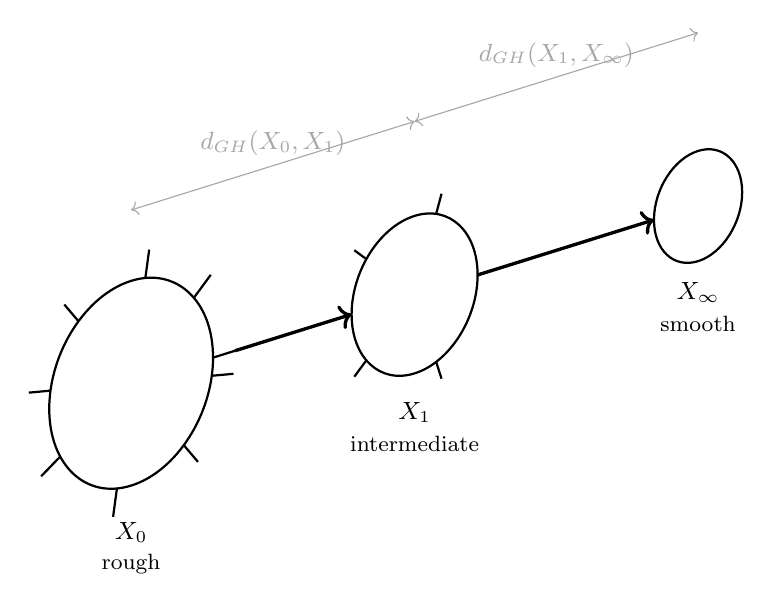
\begin{tikzpicture}[scale=1.0,
  x={({0.8cm,0.25cm})},
  y={({0cm,1cm})},
  z={({-0.5cm,0.18cm})}]
% Three "metric spaces" represented as bumpy spheres at different x-positions
% Space X0: rough/spiky (many small bumps), large radius
\def\Ra{1.3}
\draw[thick] (0,0,0) circle[radius=\Ra];
% Add irregularity spikes in 2D projection
\foreach \ang in {0,40,80,130,170,210,260,310,350} {
  \pgfmathsetmacro{\rx}{\Ra*cos(\ang)}
  \pgfmathsetmacro{\ry}{\Ra*sin(\ang)}
  \pgfmathsetmacro{\ex}{(\Ra+0.35)*cos(\ang)}
  \pgfmathsetmacro{\ey}{(\Ra+0.35)*sin(\ang)}
  \draw[thick] (\rx,\ry,0) -- (\ex,\ey,0);
}
\node[font=\small] at (0,-1.9,0) {$X_0$};
\node[font=\small] at (0,-2.3,0) {\footnotesize rough};
% Space X1: medium, fewer bumps
\def\Rb{1.0}
\draw[thick] (4.5,0,0) circle[radius=\Rb];
\foreach \ang in {0,70,140,220,290} {
  \pgfmathsetmacro{\rx}{\Rb*cos(\ang)}
  \pgfmathsetmacro{\ry}{\Rb*sin(\ang)}
  \pgfmathsetmacro{\ex}{(\Rb+0.25)*cos(\ang)}
  \pgfmathsetmacro{\ey}{(\Rb+0.25)*sin(\ang)}
  \draw[thick] (4.5+\rx,\ry,0) -- (4.5+\ex,\ey,0);
}
\node[font=\small] at (4.5,-1.5,0) {$X_1$};
\node[font=\small] at (4.5,-1.9,0) {\footnotesize intermediate};
% Space Xinfty: smooth sphere
\def\Rc{0.7}
\draw[thick] (9,0,0) circle[radius=\Rc];
\node[font=\small] at (9,-1.1,0) {$X_\infty$};
\node[font=\small] at (9,-1.5,0) {\footnotesize smooth};
% Arrows connecting them
\draw[->,very thick] (1.65,0,0) -- (3.5,0,0);
\draw[->,very thick] (5.5,0,0) -- (8.3,0,0);
% GH distance braces
\draw[<->,gray!70] (0,2.2,0) -- (4.5,2.2,0)
  node[midway,above,font=\small] {$d_{GH}(X_0,X_1)$};
\draw[<->,gray!70] (4.5,2.2,0) -- (9,2.2,0)
  node[midway,above,font=\small] {$d_{GH}(X_1,X_\infty)$};
\end{tikzpicture}
\caption{Gromov--Hausdorff convergence of plenum configurations.
The metric space $X_0$ represents an initial rough, fluctuating
plenum geometry. Entropy-driven smoothing progressively reduces
the Gromov--Hausdorff distance, yielding the intermediate state
$X_1$ and eventually the entropy-coherent attractor $X_\infty$.
The spikes indicate microscopic inhomogeneities that are
progressively absorbed.}
\end{figure}

\section{Covariant Relativistic Formulation of RSVP Dynamics}

To connect RSVP with relativistic physics, we express the plenum
dynamics in covariant form \cite{MisnerThorneWheeler,Wald}. With
spacetime coordinates $x^\mu$ and metric $g_{\mu\nu}$, the flow field
becomes a four-vector $v^\mu(x^\mu)$ and the fields $\Phi$, $S$
remain scalars. A relativistic RSVP action is
\begin{equation}
\mathcal{A} = \int d^4x\,\sqrt{-g}\;
\mathcal{L}(\Phi, v^\mu, S),
\end{equation}
with
\begin{equation}
\mathcal{L} =
\frac{1}{2}\nabla_\mu\Phi\,\nabla^\mu\Phi
+ \frac{1}{2}\rho(\Phi)\,v_\mu v^\mu
+ \frac{1}{2}\alpha\,\nabla_\mu S\,\nabla^\mu S
+ \lambda_1 S\,\nabla_\mu v^\mu
+ \lambda_2 \Phi S
- V(\Phi,S).
\end{equation}
The Euler--Lagrange equations yield
\begin{align}
\nabla_\mu \nabla^\mu \Phi &= \frac{\partial V}{\partial \Phi} - \lambda_2 S,
\label{eq:cov-phi} \\
\rho(\Phi)\,v^\mu + \lambda_1\,\nabla^\mu S &= 0,
\label{eq:cov-v} \\
\nabla_\mu \nabla^\mu S &= -\lambda_1\,\nabla_\mu v^\mu + \frac{\partial V}{\partial S}.
\label{eq:cov-S}
\end{align}
In regimes where coherent field configurations emerge, the effective
geometry perceived by observers may resemble curved spacetime,
suggesting a pathway toward recovering gravitational phenomena as
collective behavior of the plenum fields.

\section{Observable Cosmological Consequences}

For RSVP to function as a physical theory it must produce observable
predictions differing from standard cosmology.

Within the RSVP framework, photons propagating through a slowly
evolving plenum may lose energy according to
\begin{equation}
\frac{dE}{dt} = -\gamma\,\nabla S \cdot \mathbf{v},
\end{equation}
producing an effective redshift
\begin{equation}
1+z = \exp\!\left(\int \gamma\,\nabla S \cdot \mathbf{v}\;dt\right).
\end{equation}
This mechanism associates cosmological redshift with entropy-driven
energy redistribution rather than metric expansion.

Density gradients in the $\Phi$ field could also bend photon
trajectories, producing gravitational lensing effects without requiring
fundamental spacetime curvature. Entropy-driven smoothing may
furthermore influence the formation of cosmic structure, offering
alternative explanations for large-scale clustering patterns observed
in galaxy surveys. Future work must determine whether these predictions
can be made quantitatively consistent with cosmological data
\cite{Carroll2019,MisnerThorneWheeler,Penrose}.

\section{Homogeneous and Isotropic Cosmological Limit}
\label{sec:cosmo}

To connect RSVP dynamics with large-scale cosmology, we consider the
homogeneous and isotropic limit of the plenum fields. The purpose of
this reduction is not to impose a standard Friedmann--Lema\^{\i}tre--Robertson--Walker
geometry at the outset, but to show how an effective cosmological
description may arise from symmetry-restricted plenum dynamics.

\subsection{Symmetry Reduction of the Plenum Fields}

On sufficiently large scales, assume that the plenum is spatially
homogeneous and isotropic. Then the scalar density and entropy fields
depend only on time,
\begin{equation}
\Phi = \Phi(t), \qquad S = S(t),
\end{equation}
and in a comoving frame the flow field takes the form $v^\mu =
(v^0(t),0,0,0)$, so that spatial gradients vanish.

\subsection{Effective Cosmological Metric}

The emergent metric ansatz reduces to a diagonal form
\begin{equation}
ds^2 = -N^2(t)\,dt^2 + a^2(t)\,\delta_{ij}\,dx^i dx^j,
\end{equation}
where $a^2(t) = A(\Phi,S)$ is the derived scale factor and $N^2(t)$
incorporates flow and entropy-rate corrections. The effective
cosmological scale factor is thus a collective variable derived from
the scalar and entropy content of the plenum.

\subsection{Friedmann-Like Equations}

Varying the symmetry-reduced action and expressing dynamics through
$a(t)$ yields a Friedmann-like relation,
\begin{equation}
H^2 = \frac{\kappa_{\mathrm{eff}}}{3}\,\rho_{\mathrm{plenum}}
+ \Delta_{\mathrm{ent}},
\end{equation}
where $H = \dot{a}/a$ is the effective Hubble rate,
\begin{equation}
\rho_{\mathrm{plenum}} =
\frac{1}{2}\dot{\Phi}^2
+ \frac{1}{2}\alpha\dot{S}^2
+ \frac{1}{2}\rho(\Phi)(v^0)^2
+ V(\Phi,S) - \lambda_2\Phi S,
\end{equation}
and $\Delta_{\mathrm{ent}}$ collects correction terms arising from the
entropy--flow coupling. A parallel acceleration equation takes the form
\begin{equation}
\frac{\ddot{a}}{a} =
-\frac{\kappa_{\mathrm{eff}}}{6}
\bigl(\rho_{\mathrm{plenum}} + 3p_{\mathrm{plenum}}\bigr)
+ \Xi_{\mathrm{ent}},
\end{equation}
where $p_{\mathrm{plenum}}$ is the effective pressure generated by the
plenum fields and $\Xi_{\mathrm{ent}}$ collects entropy-driven
corrections.

\subsection{Redshift and Attractor Cosmologies}

In the RSVP framework, the quantity $a(t)$ is an emergent collective
variable, so cosmological redshift may be interpreted either as
propagation through an effective geometry with time-dependent scale
factor, or as a manifestation of entropy-driven redistribution in the
underlying plenum. A particularly important case arises when $a(t)$ is
approximately constant while the entropy and flow fields continue to
evolve: the large-scale geometry is then effectively static while
photons accumulate redshift through entropy-coupled propagation.

Because RSVP dynamics admit a gradient-flow interpretation, the
homogeneous cosmological solutions may be interpreted as trajectories
in a reduced phase space flowing toward critical points of
$\mathcal{R}$. A stationary cosmology corresponds to a critical point
satisfying $\delta\mathcal{R}/\delta\Phi =
\delta\mathcal{R}/\delta S = \delta\mathcal{R}/\delta v^0 = 0$, and
different cosmological histories correspond to different basins of
attraction.

\section{A Toy Redshift Law and Luminosity Distance}
\label{sec:redshift}

\subsection{Entropy-Driven Redshift}

Consider a photon of energy $E(t)$ propagating through a homogeneous
plenum with time-dependent entropy field $S(t)$ and flow component
$v^0(t)$. Motivated by the coupling structure of the RSVP action, the
photon energy obeys
\begin{equation}
\frac{dE}{dt} = -\gamma\,\Theta(t)\,E,
\end{equation}
where the effective attenuation rate is
\begin{equation}
\Theta(t) = \alpha_1\dot{S}(t) + \alpha_2 v^0(t) + \alpha_3\nabla_\mu v^\mu.
\end{equation}
Solving yields
\begin{equation}
1+z = \frac{E(t_{\mathrm{em}})}{E(t_{\mathrm{obs}})}
= \exp\!\left(\gamma\int_{t_{\mathrm{em}}}^{t_{\mathrm{obs}}}\Theta(t)\,dt\right).
\label{eq:toy-redshift}
\end{equation}
If $\Theta(t) = \Theta_0$ is approximately constant, then $1+z =
e^{\gamma\Theta_0\Delta t}$, reducing at small redshift to $z \approx
\gamma\Theta_0\Delta t$. If the dominant contribution is entropy
relaxation, then $1+z = \exp(\gamma\alpha_1[S(t_{\mathrm{obs}}) -
S(t_{\mathrm{em}})])$, so redshift directly measures the cumulative
entropy difference encountered during propagation.

\subsection{Luminosity Distance}

Using the standard definition $F = L/(4\pi d_L^2)$ and accounting for
both energy loss and arrival-rate suppression by a factor $(1+z)^{-2}$,
the luminosity distance is
\begin{equation}
d_L(z) = (1+z)\,r(z),
\end{equation}
where $r(z) = \int_{t_{\mathrm{em}}}^{t_{\mathrm{obs}}}
c_{\mathrm{eff}}(t)/a(t)\,dt$ is the propagation distance. In the
constant-$\Theta$ approximation,
\begin{equation}
d_L(z) = \frac{c_{\mathrm{eff}}}{\gamma\Theta_0}(1+z)\ln(1+z),
\label{eq:dl-log}
\end{equation}
with small-redshift expansion
\begin{equation}
d_L(z) \approx \frac{c_{\mathrm{eff}}}{\gamma\Theta_0}
\left(z + \frac{z^2}{2} + \mathcal{O}(z^3)\right),
\end{equation}
reproducing a linear Hubble-like law with effective scale $H_{\mathrm{eff}}
\equiv \gamma\Theta_0$.

\subsection{Modified Reciprocity Relation}

The angular-diameter distance $d_A$ is determined by the geometric
spreading of null congruences and is insensitive to entropy-driven
energy loss at leading order, giving $d_A(z) = r(z)/(1+z_{\mathrm{geom}})$.
Since the total redshift decomposes as $(1+z) = (1+z_{\mathrm{geom}})
(1+z_{\mathrm{ent}})$, one obtains the modified reciprocity relation
\begin{equation}
d_L = (1+z_{\mathrm{ent}})\,(1+z_{\mathrm{geom}})^2\,d_A.
\end{equation}
When entropy-driven attenuation is absent ($z_{\mathrm{ent}}=0$), this
reduces to the standard Etherington relation $d_L = (1+z)^2 d_A$.
Precision measurements comparing luminosity distances and
angular-diameter distances therefore provide a direct test of the RSVP
framework: any systematic deviation from the standard $(1+z)^2$ ratio
signals the presence of non-metric contributions to redshift.

\section{Parameter Estimation Framework for RSVP Cosmology}
\label{sec:paramest}

\subsection{Parametrization}

We introduce a minimal parametrization of the attenuation rate as a
function of redshift,
\begin{equation}
\Theta(z) = H_0 + \beta z + \mathcal{O}(z^2),
\end{equation}
where $H_0$ plays the role of an effective Hubble scale and $\beta$
captures deviations from linear behavior. The luminosity distance
becomes
\begin{equation}
d_L(z;\theta) =
(1+z)\int_0^z \frac{c_{\mathrm{eff}}}{\gamma\Theta(z')}\,dz',
\end{equation}
where $\theta = (H_0,\beta,\ldots)$ is the parameter vector. For the
simplest case $\Theta = H_0$, this reduces to
equation~(\ref{eq:dl-log}). The corresponding distance modulus is
\begin{equation}
\mu(z;\theta) = 5\log_{10}\!\left(\frac{d_L(z;\theta)}{10\,\mathrm{pc}}\right).
\end{equation}

\subsection{Likelihood and Comparison with $\Lambda$CDM}

Given a dataset of supernovae $\{z_i,\mu_i,\sigma_i\}$, a Gaussian
likelihood takes the standard form
\begin{equation}
\mathcal{L}(\theta) \propto \exp\!\left(
-\frac{1}{2}\sum_i\frac{[\mu_i - \mu(z_i;\theta)]^2}{\sigma_i^2}
\right).
\end{equation}
In the standard $\Lambda$CDM model, the luminosity distance is
\begin{equation}
d_L^{\Lambda\mathrm{CDM}}(z) = (1+z)\int_0^z\frac{c}{H(z')}\,dz',
\end{equation}
with $H(z)$ determined by the Friedmann equations. The RSVP model
replaces the expansion rate $H(z)$ with the attenuation function
$\gamma\Theta(z)$, yielding the same integral structure but a
different physical interpretation. Both models can be fitted to the
same datasets and compared by standard model-selection criteria.

At low redshift, the RSVP model mimics the standard linear Hubble law.
At higher redshift, the logarithmic corrections in equation~(\ref{eq:dl-log})
predict deviations from $\Lambda$CDM that grow with $z$ and can in
principle be distinguished using supernova, baryon acoustic oscillation,
and cosmic chronometer data. Violations of the standard reciprocity
relation provide an additional independent diagnostic.

\section{Emergent Metric Structure from Plenum Fields}
\label{sec:emergentmetric}

\subsection{Effective Metric Ansatz}

To establish a connection between RSVP dynamics and geometric
descriptions of spacetime, we construct an effective metric from the
plenum fields. A natural symmetric rank-2 tensor built from the
available field content is
\begin{equation}
g_{\mu\nu}^{\mathrm{eff}} =
A(\Phi,S)\,\eta_{\mu\nu}
+ B(\Phi,S)\,v_\mu v_\nu
+ C(\Phi,S)\,\nabla_\mu S\,\nabla_\nu S,
\end{equation}
where $\eta_{\mu\nu}$ is the background Minkowski metric and
$A,B,C$ are scalar functions encoding how density and entropy modify
effective geometry. The first term represents isotropic scaling
determined by the local plenum state; the second and third terms
introduce anisotropy due to flow and entropy gradients.

\subsection{Metric as a Pullback from Field Space}

A more fundamental origin of this metric arises from the pullback
construction. At each spacetime point $x^\mu$, the fields define a
map $X : x^\mu \mapsto X^A(x^\mu)$ from spacetime into the plenum
configuration space $\mathcal{M}$. The effective spacetime metric is
then obtained as the pullback of the field-space metric $G_{AB}$
along this map:
\begin{equation}
g_{\mu\nu}^{\mathrm{eff}} =
G_{AB}(X)\,\partial_\mu X^A\,\partial_\nu X^B,
\end{equation}
giving schematically
\begin{equation}
g_{\mu\nu}^{\mathrm{eff}} \sim
(\partial_\mu\Phi)(\partial_\nu\Phi)
+ \rho(\Phi)(\partial_\mu v^\alpha)(\partial_\nu v_\alpha)
+ \alpha(\partial_\mu S)(\partial_\nu S) + \cdots
\end{equation}
The ansatz from the previous subsection is a low-order approximation
to this pullback, obtained by truncating higher-derivative terms. This
construction is analogous to induced metrics in sigma models, and it
unifies the geometric and dynamical aspects of RSVP: the same metric
$G_{AB}$ governs both gradient flow in field space and the induced
geometry of spacetime.

\subsection{Induced Connection and Effective Field Equations}

Given $g_{\mu\nu}^{\mathrm{eff}}$, the Levi-Civita connection and
curvature tensor are derived quantities reflecting spatial and temporal
variations of the plenum fields. In a slow-variation regime where
higher-order derivative terms may be neglected, variation of the
effective action with respect to the metric yields an equation of the
form
\begin{equation}
G_{\mu\nu}(g_{\mathrm{eff}}) =
\kappa_{\mathrm{eff}}\,T_{\mu\nu}^{(\Phi,v,S)}
+ \mathcal{O}(\nabla^2 X),
\end{equation}
where $T_{\mu\nu}^{(\Phi,v,S)}$ is the effective stress-energy tensor
built from the plenum fields and $\kappa_{\mathrm{eff}}$ is an
effective coupling. This has the same structural form as Einstein's
field equations, but with both metric and stress-energy arising from
the same underlying plenum fields. In regimes where entropy gradients
are small and flow is negligible, the metric reduces to a conformally
rescaled form $g_{\mu\nu}^{\mathrm{eff}} \approx A(\Phi)\,\eta_{\mu\nu}$
and the equations reduce to scalar-field-driven gravity models. More
general configurations introduce anisotropic and dissipative
corrections leading to deviations from standard general relativity.

\section{Lattice Discretization of RSVP Field Dynamics}

Because the RSVP equations resemble nonlinear transport and diffusion
systems, lattice discretization provides a practical route to numerical
exploration. On a cubic lattice with spacing $\Delta x$ and time step
$\Delta t$, the scalar density field is represented at lattice sites
$\Phi_{i,j,k}(t)$, vector flow components are stored on lattice edges
$v^x_{i+1/2,j,k}$, $v^y_{i,j+1/2,k}$, $v^z_{i,j,k+1/2}$, and the
entropy field at lattice sites $S_{i,j,k}(t)$. The discretized
evolution equations are
\begin{align}
\Phi_{i,j,k}^{t+1} &= \Phi_{i,j,k}^t
+ \Delta t\left(-\nabla_h\cdot(\Phi\mathbf{v})
+ D_\Phi\,\nabla_h^2\Phi\right), \\
S_{i,j,k}^{t+1} &= S_{i,j,k}^t
+ \Delta t\left(-\nabla_h\cdot(S\mathbf{v})
+ D_S\,\nabla_h^2 S + \sigma\right),
\end{align}
where $\nabla_h$ denotes the discrete spatial derivative.
Vector flow dynamics are evolved using discretized vorticity and
pressure-gradient terms derived from the RSVP action. Such lattice
simulations may reveal emergent phenomena including entropy-driven
smoothing of density fluctuations, formation of coherent flow
structures, and long-range correlations resembling gravitational
clustering.

\begin{figure}[H]
\centering
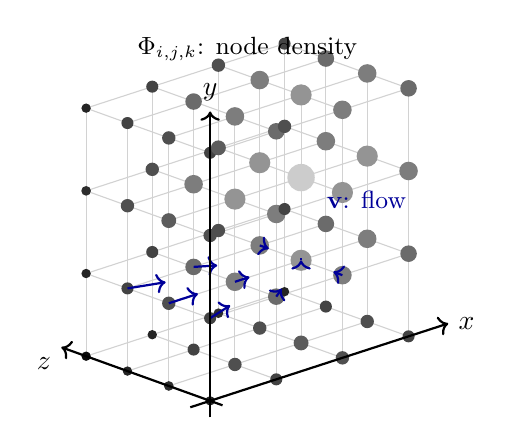
\begin{tikzpicture}[scale=1.05,
  x={({0.8cm,0.26cm})},
  y={({0cm,1cm})},
  z={({-0.5cm,0.18cm})}]
% 4x4x4 lattice nodes
\def\N{3}
% Draw lattice edges
\foreach \xi in {0,...,\N} {
  \foreach \zi in {0,...,\N} {
    \draw[gray!35,thin] (\xi,0,\zi) -- (\xi,\N,\zi);
  }
}
\foreach \yi in {0,...,\N} {
  \foreach \zi in {0,...,\N} {
    \draw[gray!35,thin] (0,\yi,\zi) -- (\N,\yi,\zi);
  }
}
\foreach \xi in {0,...,\N} {
  \foreach \yi in {0,...,\N} {
    \draw[gray!35,thin] (\xi,\yi,0) -- (\xi,\yi,\N);
  }
}
% Lattice sites: filled circles, shaded by a fake Phi value
% High density cluster near (2,2,1)
\foreach \xi in {0,...,\N} {
  \foreach \yi in {0,...,\N} {
    \foreach \zi in {0,...,\N} {
      \pgfmathsetmacro{\dist}{sqrt((\xi-2)*(\xi-2)+(\yi-2)*(\yi-2)+(\zi-1)*(\zi-1))}
      \pgfmathsetmacro{\sz}{max(1.2, 3.5 - 0.8*\dist)}
      \pgfmathsetmacro{\gr}{min(100, 20 + 22*\dist)}
      \node[circle,fill=black!\gr!white,inner sep=\sz pt] at (\xi,\yi,\zi) {};
    }
  }
}
% Vector flow arrows on a central slice (yi=1)
\foreach \xi in {0,1,2} {
  \foreach \zi in {0,1,2} {
    \pgfmathsetmacro{\dx}{(2-\xi)*0.22}
    \pgfmathsetmacro{\dz}{(1-\zi)*0.22}
    \draw[->,thick,blue!60!black]
      (\xi,1,\zi) -- ({\xi+\dx},1,{\zi+\dz});
  }
}
% Axis labels
\draw[->,thick] (-0.3,0,0) -- (\N+0.6,0,0) node[right] {$x$};
\draw[->,thick] (0,-0.2,0) -- (0,\N+0.5,0) node[above] {$y$};
\draw[->,thick] (0,0,-0.3) -- (0,0,\N+0.6) node[below left] {$z$};
% Field labels
\node[font=\small] at (1.5,\N+0.6,1.5) {$\Phi_{i,j,k}$: node density};
\node[font=\small,blue!60!black] at (\N+0.3,1.3,1.5) {$\mathbf{v}$: flow};
\end{tikzpicture}
\caption{Lattice discretization of the RSVP plenum. Node shading
encodes the scalar density field $\Phi_{i,j,k}$: darker nodes indicate
higher density, forming a coherent cluster near the lattice center.
Blue arrows on the central horizontal slice show vector flow field
components $\mathbf{v}$, here directed inward toward the density peak.
The entropy field $S_{i,j,k}$ is defined at each site and evolved
simultaneously using the discretized advection--diffusion equation.}
\end{figure}


\section{Future Directions}

The RSVP framework remains at an early conceptual stage and requires
substantial mathematical and empirical development before it can be
considered a predictive physical theory.

\subsection{Mathematical Development}

A first priority is the construction of a fully consistent dynamical
theory for the plenum fields $(\Phi,\mathbf{v},S)$. The action
functional introduced above should be generalized to ensure full
covariance, stability of solutions, and compatibility with known
physical constraints. Key open questions include the geometric structure
of the configuration manifold; the existence of monotonic
entropy--coherence functionals; classification of stationary solutions
and attractor regimes; and the precise relationship between RSVP
gradient flows and renormalization group dynamics.

\subsection{Connections with Quantum Field Theory}

A precise correspondence between RSVP field dynamics and conventional
quantum field theory requires explicit coarse-graining maps between
microscopic field theories and the RSVP plenum variables. One
possibility is that RSVP dynamics arise as a coarse-grained description
of deeper microscopic degrees of freedom, in much the same way that
hydrodynamics emerges from molecular physics.

\subsection{Numerical Simulation}

Lattice-based simulations could model the coupled evolution of
$\Phi$, $\mathbf{v}$, and $S$ under simplified dynamical rules.
Such simulations may reveal emergent phenomena including
self-organizing flow structures, entropy-driven smoothing of density
fluctuations, and long-range coherence patterns resembling
gravitational clustering.

\subsection{Cosmological Observables}

Possible avenues for observational testing include alternative
interpretations of cosmological redshift, entropy-based explanations
for large-scale structure formation, modified predictions for
gravitational lensing patterns, and deviations from standard cosmic
expansion histories.

\subsection{Conceptual Foundations}

If spacetime geometry emerges from entropy-driven plenum dynamics, the
fundamental ontology of physics may shift from geometric objects to
informational and thermodynamic processes. Exploring this possibility
could clarify the relationship between gravity, information, and the
large-scale structure of the universe \cite{Butterfield,Seiberg,
Penrose,Carroll2022}.

\section{Structural Convergence Without Derivation}
\label{sec:convergence}

The preceding sections develop a formal framework in which physical
structure emerges from local interactions, entropy-driven dynamics, and
variational principles. An important implication of this perspective
concerns the way complex theoretical expressions are generated,
interpreted, and evaluated.

It is a recurring phenomenon in theoretical work that expressions of
considerable structural similarity arise independently across different
contexts. Functional derivatives of effective actions, entropy terms,
renormalization group flows, and nonlocal kernels appear naturally in
quantum field theory, statistical mechanics, and information-theoretic
approaches to physics.

From the RSVP perspective, this convergence is not accidental. It
reflects the fact that many systems---physical, computational, and
cognitive---are governed by common principles combining local variation,
global consistency, and entropy constraints. As a result, expressions
that bring together effective actions, functional derivatives, entropy
contributions, and flow constraints tend to reappear as structurally
stable attractors in the space of possible formalisms.

Within the Spherepop interpretation, such expressions may be understood
as high-level configurations toward which symbolic systems evolve under
constraints of coherence and compression. However, the existence of
such attractors does not guarantee that a given expression encodes a
well-defined or empirically meaningful theory. Distinct derivations may
lead to superficially similar forms while differing fundamentally in
interpretation, domain of validity, and predictive content.

Scientific practice places central importance on derivation, not merely
on final expressions. A formula acquires meaning through the sequence
of transformations, approximations, and assumptions that produce it.
Formally, this may be expressed as a mapping
\begin{equation}
\mathcal{D} : \text{assumptions} \longrightarrow \text{equations},
\end{equation}
where the derivation $\mathcal{D}$ encodes the structure necessary for
reproducibility and comparison. Without this mapping, an expression
remains underdetermined, admitting multiple incompatible
interpretations or failing to connect to any well-defined dynamical
system.

This phenomenon has implications for both human and machine-generated
theoretical work. In particular, the appearance of a highly structured
expression should not be taken as evidence of a unified theory in the
absence of a transparent derivation. Within RSVP, this is understood
as a distinction between \emph{structural plausibility}---convergence
toward common symbolic patterns---and \emph{derivational validity}---the
existence of a well-defined generative process linking assumptions to
predictions.

\section{Derivation as a Path in Theory Space}
\label{sec:derivationpath}

We now make the notion of derivation precise by modeling it as a path
in a suitably defined space of theories \cite{Zamolodchikov1986,
PannellStergiou2025}.

Let $\mathcal{T}$ denote the space of admissible theoretical
configurations, where a point $\tau \in \mathcal{T}$ consists of a
specification of fields, symmetries, action functional, and
constraints:
\begin{equation}
\tau = (\mathcal{F}, \mathcal{S}, \mathcal{A}, \mathcal{C}).
\end{equation}
A derivation is then a path in theory space,
\begin{equation}
\gamma : [0,1] \rightarrow \mathcal{T},
\end{equation}
with $\gamma(0) = \tau_{\mathrm{initial}}$ and $\gamma(1) =
\tau_{\mathrm{final}}$. Each infinitesimal segment of the path
corresponds to a well-defined transformation---variation, coarse-graining,
field redefinition, symmetry reduction, or quantization---so derivation
is not merely a sequence of symbolic steps but a structured trajectory
through the space of admissible theories.

Different derivations may lead to the same final expression while
traversing distinct regions of theory space, explaining why
structurally similar equations arise from different theoretical contexts
while encoding different physics. The derivation process may be
formalized as a functor
\begin{equation}
\mathcal{D} : \mathcal{C}_{\mathrm{assumptions}}
\rightarrow \mathcal{C}_{\mathrm{theories}},
\end{equation}
mapping a category of assumptions and transformations to a category of
resulting theories, with composition of transformations corresponding
to composition of morphisms.

Within the Spherepop framework, derivations correspond to event
histories: each transformation along $\gamma$ is represented by a
discrete event $e_i$, so
\begin{equation}
\gamma \;\longleftrightarrow\; (e_1, e_2, \ldots, e_n).
\end{equation}
A valid derivation therefore corresponds to a well-formed event trace,
while an isolated expression without history corresponds to a terminal
state with no accessible generative path.

To quantify proximity between theories, one equips $\mathcal{T}$ with
a metric or divergence functional $d(\tau_1,\tau_2)$ measuring
differences in predictions, symmetries, or information content. Paths
minimizing this functional correspond to efficient derivations,
analogous to geodesics in theory space. This connects naturally to
renormalization group flows, which may be interpreted as gradient flows
with respect to such a metric \cite{Zamolodchikov1986,PannellStergiou2025}.

\section{Homotopy Classes of Derivations}
\label{sec:homotopy}

Having modeled derivations as paths in theory space, we now refine this
structure by introducing an equivalence relation based on continuous
deformation.

Let $\gamma_1, \gamma_2 : [0,1] \to \mathcal{T}$ be two derivations
connecting the same initial and final theories. We say that $\gamma_1$
and $\gamma_2$ are \emph{homotopic} if there exists a continuous family
\begin{equation}
H : [0,1]\times[0,1] \to \mathcal{T}
\end{equation}
with $H(s,0) = \gamma_1(s)$, $H(s,1) = \gamma_2(s)$,
$H(0,t) = \tau_{\mathrm{initial}}$, and $H(1,t) = \tau_{\mathrm{final}}$
for all $t$. Two derivations are thus equivalent if one can be
continuously deformed into the other without leaving the space of
admissible theories.

The set of equivalence classes $[\gamma]$ under homotopy captures the
essential structure of a derivation independent of inessential choices
such as intermediate parameterizations or auxiliary representations.
From a physical standpoint, two derivations are equivalent if they
correspond to transformations that preserve all observable predictions,
as with field redefinitions, gauge transformations, and changes of
renormalization scheme.

Not all derivations connecting the same endpoints are homotopic.
Obstructions may arise from topological features of theory space or
from singularities encountered along intermediate steps, indicating
genuine distinctions between theories that cannot be removed by
continuous deformation.

The collection of theories and derivations naturally forms a higher
categorical structure: theories are objects, derivations are
1-morphisms, and homotopies between derivations are 2-morphisms.
Iterating this construction leads to an $\infty$-groupoid of theories
in which all higher equivalences are encoded systematically
\cite{LurieTFT}. Within Spherepop, homotopies between derivations
correspond to transformations of event sequences that preserve overall
outcomes, so homotopy classes of derivations correspond to equivalence
classes of event traces.

\section{Variational Principles on Theory Space}
\label{sec:variationaltheory}

We now complete the framework by defining a variational principle on
the space of derivations.

Define a functional $\mathcal{S}_{\mathrm{der}}[\gamma]$ assigning a
cost to each derivation path:
\begin{equation}
\mathcal{S}_{\mathrm{der}}[\gamma]
= \int_0^1
\Bigl[
\lambda_1 \|\dot{\gamma}(s)\|^2
+ \lambda_2\,\mathcal{U}(\gamma(s))
+ \lambda_3\,\mathcal{I}(\gamma(s))
\Bigr]\, ds,
\end{equation}
where $\|\dot{\gamma}\|$ measures the rate of change in theory space,
$\mathcal{U}$ is a potential encoding inconsistency or instability, and
$\mathcal{I}$ measures informational cost. A valid or optimal
derivation is a path that extremizes $\mathcal{S}_{\mathrm{der}}$:
\begin{equation}
\delta\mathcal{S}_{\mathrm{der}}[\gamma] = 0.
\end{equation}
Such paths are geodesics in theory space with respect to an effective
metric induced by the functional, representing the most efficient
transformations between theories under the chosen criteria.

In many cases this functional induces a gradient flow
\begin{equation}
\frac{d\gamma^A}{ds} = -G^{AB}\frac{\partial\mathcal{F}}{\partial\gamma^B},
\end{equation}
which is directly parallel to the RSVP dynamics of plenum fields,
establishing a correspondence between physical evolution and the
evolution of theoretical descriptions. The informational term
$\mathcal{I}$ may be interpreted as measuring the entropy or complexity
of intermediate representations: paths that introduce unnecessary
structure incur higher cost, while paths maintaining coherence are
favored. This aligns with the RSVP interpretation of physical dynamics
as entropy-constrained evolution.

The existence of a variational principle explains why certain formal
structures recur across different contexts. These structures correspond
to low-action regions in theory space, making them natural endpoints of
many distinct derivational paths---but a low-action endpoint does not
uniquely determine the path taken to reach it, reinforcing the
necessity of explicit derivational specification.

\section{Constraint Before Content}
\label{sec:constraintcontent}

The preceding development has introduced a layered framework in which
physical systems, symbolic structures, and theoretical constructions
are all described in terms of constrained evolution. We articulate the
unifying principle underlying these constructions.

In traditional formulations, physical theories are presented in terms
of objects---fields, particles, or states---together with equations
governing their behavior. The RSVP framework suggests instead that
constraint is primary, and that objects arise as secondary
manifestations of constraint satisfaction. The dynamics of the plenum
are governed by
\begin{equation}
\delta\mathcal{R} = 0,
\end{equation}
which determines admissible configurations of the fields
$(\Phi,\mathbf{v},S)$. Spacetime geometry, matter distributions, and
interaction patterns are emergent solutions to this constraint, not
independently specified inputs.

An analogous structure appears at the level of theory construction.
Derivations are paths $\gamma \subset \mathcal{T}$ constrained by
consistency, coherence, and informational criteria. The variational
principle
\begin{equation}
\delta\mathcal{S}_{\mathrm{der}}[\gamma] = 0
\end{equation}
selects preferred derivations, while homotopy classes organize
equivalences between them. Theoretical objects---equations, models,
and formalisms---are endpoints of constrained processes in theory
space, not primitive entities.

This principle manifests in both continuous and discrete settings: in
RSVP through gradient flows in field space, in Spherepop through
admissible event histories. In both frameworks, valid states arise from
sequences of transformations subject to global consistency conditions.

The recurrence of similar formal structures across independent
contexts---whether in physics, computation, or symbolic
reasoning---follows from shared constraint landscapes. Certain
configurations act as attractors because they satisfy these constraints
efficiently. This explains the convergence of complex expressions
across different derivations, while clarifying why such convergence
does not, by itself, establish theoretical equivalence.

Across all levels of description, structure arises not as a primitive
given but as the outcome of constrained evolution. Physical systems
evolve along paths minimizing an action functional; theoretical
derivations follow paths minimizing a derivational cost; symbolic
systems organize themselves under constraints of coherence and entropy.
In this sense the distinction between physics, computation, and theory
construction becomes one of representation rather than principle:
constraint precedes content, and content emerges as its realization.

\section{Conclusion}

Renormalization group theory, effective action methods, and entropy-based
approaches to gravity all emphasize the role of information flow in
shaping physical laws. The RSVP framework extends this perspective by
proposing that the universe itself may evolve through entropy-driven
field dynamics within a plenum.

We have derived the RSVP field equations from a candidate action
functional, established conservation laws, analyzed linear stability,
and connected the framework to renormalization group theory, asymptotic
safety, holographic renormalization, sheaf-theoretic locality, derived
geometry, and Gromov--Hausdorff convergence. The structural similarities
between RG flow and RSVP evolution are not merely analogical but suggest
that modern quantum field theory may already contain the mathematical
tools needed to formalize such a framework.

Further work is needed to establish rigorous derivations, make contact
with empirical predictions, and explore the connections with derived
algebraic geometry and categorical field theory.

\newpage
\section*{Appendices}
\addcontentsline{toc}{section}{Appendices}

\appendix

\section{Notation and Symbol Glossary}

For clarity, we summarize the principal symbols used throughout this
manuscript.

\medskip
\begin{center}
\begin{tabular}{@{} p{0.27\textwidth} p{0.62\textwidth} @{}}
\toprule
Symbol & Meaning \\
\midrule
$\Phi(x,t)$ & Scalar density field of the plenum \\
$\mathbf{v}(x,t)$ & Vector flow field describing directional transport \\
$S(x,t)$ & Entropy field governing thermodynamic redistribution \\
$\mathcal{A}_{RSVP}$ & Action functional defining plenum dynamics \\
$\mathcal{L}$ & Lagrangian density of the RSVP theory \\
$\mathcal{R}$ & Entropy--coherence functional generating gradient flow \\
$G^{AB}$ & Metric on plenum field configuration space \\
$g_i$ & Coupling constants in renormalization group theory \\
$\Gamma_{\text{eff}}$ & Effective quantum action \\
$\Gamma_k$ & Wilsonian effective action at scale $k$ \\
$G_{ij}$ & Zamolodchikov metric on theory space \\
$H$ & Helicity invariant of the vector flow field \\
$d_{GH}$ & Gromov--Hausdorff distance between metric spaces \\
$E_r^{p,q}$ & Spectral sequence terms for scale cascade \\
$\mathcal{P}$ & Sheaf of plenum field configurations \\
$\mathcal{C}_\lambda$ & Coarse-graining functor on plenum states \\
$\omega_{BV}$ & BV odd symplectic form on extended field space \\
$\Pi_\Phi$, $\boldsymbol{\Pi}_v$, $\Pi_S$ & Canonical momenta of plenum fields \\
$\lambda_1$, $\lambda_2$, $\lambda_3$ & Interaction coupling constants \\
\bottomrule
\end{tabular}
\end{center}

\section{Core Mathematical Results}
\label{app:theorems}

\begin{theorem}[Gradient Flow Structure]
\label{thm:gradient}
Let $\mathcal{R}[\Phi,\mathbf{v},S]$ be the entropy--coherence
functional defined on plenum field space with $G^{AB}$ a positive
definite metric. If the field dynamics satisfy
\begin{equation}
\partial_t X^A = -G^{AB}\frac{\delta \mathcal{R}}{\delta X^B},
\end{equation}
then $\mathcal{R}$ is non-increasing along solution trajectories.
\end{theorem}

\begin{proof}
Computing the time derivative of $\mathcal{R}$ yields
\begin{equation}
\frac{d\mathcal{R}}{dt} =
\int \frac{\delta \mathcal{R}}{\delta X^A}\,\partial_t X^A\, d^3x.
\end{equation}
Substituting the gradient flow equation gives
\begin{equation}
\frac{d\mathcal{R}}{dt} =
-\int G^{AB}
\frac{\delta \mathcal{R}}{\delta X^A}
\frac{\delta \mathcal{R}}{\delta X^B}\, d^3x.
\end{equation}
Positive definiteness of $G^{AB}$ implies the integrand is
non-negative pointwise, so
\begin{equation}
\frac{d\mathcal{R}}{dt} \leq 0,
\end{equation}
with equality if and only if $\delta\mathcal{R}/\delta X^A = 0$
everywhere.
\end{proof}

\begin{proposition}[Stationary Plenum States]
Configurations satisfying
\begin{equation}
\frac{\delta \mathcal{R}}{\delta X^A} = 0
\end{equation}
correspond to stationary solutions of the RSVP field equations and
to critical points of the entropy--coherence functional.
\end{proposition}

\begin{proposition}[Scale Hierarchy and Effective Flow]
If the plenum fields admit a multiscale decomposition
\begin{equation}
X = \sum_k X_k
\end{equation}
via the Fourier expansion, then coarse-graining transformations
\begin{equation}
X \mapsto \bar{X}_\Lambda = \int_{|k|<\Lambda}\tilde{X}(k)\,e^{ikx}\,d^3k
\end{equation}
define a renormalization-like flow on the space of effective plenum
descriptions, with the infrared limit corresponding to stationary
plenum regimes.
\end{proposition}

\begin{proposition}[Entropy Monotonicity]
Let $\sigma \geq 0$. Then the total entropy $\int S\,d^3x$ is
non-decreasing along solutions of the RSVP entropy balance equation,
consistent with the second law of thermodynamics.
\end{proposition}

\section{Step-by-Step Derivation of the Covariant Field Equations}

For completeness we derive the covariant RSVP field equations
(\ref{eq:cov-phi})--(\ref{eq:cov-S}) in detail.

The covariant Lagrangian is
\begin{equation}
\mathcal{L} =
\frac{1}{2}\nabla_\mu\Phi\,\nabla^\mu\Phi
+ \frac{1}{2}\rho(\Phi)\,v_\mu v^\mu
+ \frac{1}{2}\alpha\,\nabla_\mu S\,\nabla^\mu S
+ \lambda_1 S\,\nabla_\mu v^\mu
+ \lambda_2\,\Phi S
- V(\Phi,S).
\end{equation}

\subsection*{Variation with respect to $\Phi$}

The terms in $\mathcal{L}$ depending on $\Phi$ or $\nabla_\mu\Phi$
are
\begin{equation}
\frac{1}{2}\nabla_\mu\Phi\,\nabla^\mu\Phi
+ \frac{1}{2}\frac{d\rho}{d\Phi}\,v_\mu v^\mu\,\Phi
+ \lambda_2\,\Phi S - V(\Phi,S).
\end{equation}
The Euler--Lagrange equation
$\nabla_\mu(\partial\mathcal{L}/\partial(\nabla_\mu\Phi))
= \partial\mathcal{L}/\partial\Phi$
gives
\begin{equation}
\nabla_\mu\nabla^\mu\Phi =
\frac{\partial V}{\partial\Phi} - \lambda_2 S.
\end{equation}

\subsection*{Variation with respect to $v^\mu$}

The dependence on $v^\mu$ is
\begin{equation}
\frac{1}{2}\rho(\Phi)\,v_\mu v^\mu + \lambda_1 S\,\nabla_\mu v^\mu.
\end{equation}
Integrating by parts in the action to move the derivative off $v^\mu$,
the Euler--Lagrange equation yields
\begin{equation}
\rho(\Phi)\,v^\mu + \lambda_1\,\nabla^\mu S = 0.
\end{equation}

\subsection*{Variation with respect to $S$}

The terms depending on $S$ or $\nabla_\mu S$ are
\begin{equation}
\frac{1}{2}\alpha\,\nabla_\mu S\,\nabla^\mu S
+ \lambda_1 S\,\nabla_\mu v^\mu + \lambda_2\,\Phi S - V(\Phi,S).
\end{equation}
The Euler--Lagrange equation gives
\begin{equation}
\alpha\,\nabla_\mu\nabla^\mu S =
-\lambda_1\,\nabla_\mu v^\mu - \lambda_2\,\Phi
+ \frac{\partial V}{\partial S}.
\end{equation}
Setting $\alpha = 1$ these reproduce equations
(\ref{eq:cov-phi})--(\ref{eq:cov-S}).

\begin{thebibliography}{99}

\bibitem{Wilson1974}
K.~G.~Wilson and J.~Kogut,
\emph{The Renormalization Group and the $\epsilon$ Expansion},
Physics Reports \textbf{12}, 75--199 (1974).

\bibitem{Zamolodchikov1986}
A.~B.~Zamolodchikov,
\emph{Irreversibility of the Flux of the Renormalization Group in a 2D Field Theory},
JETP Letters \textbf{43}, 730--732 (1986).

\bibitem{Weinberg1979}
S.~Weinberg,
\emph{Ultraviolet Divergences in Quantum Theories of Gravitation},
in \emph{General Relativity: An Einstein Centenary Survey},
Cambridge University Press (1979).

\bibitem{Reuter1998}
M.~Reuter,
\emph{Nonperturbative Evolution Equation for Quantum Gravity},
Physical Review D \textbf{57}, 971--985 (1998).

\bibitem{PannellStergiou2025}
W.~H.~Pannell and A.~Stergiou,
\emph{Gradient Flows and the Curvature of Theory Space},
arXiv:2502.06940 (2025).

\bibitem{Jacobson1995}
T.~Jacobson,
\emph{Thermodynamics of Spacetime: The Einstein Equation of State},
Physical Review Letters \textbf{75}, 1260--1263 (1995).

\bibitem{Verlinde2011}
E.~Verlinde,
\emph{On the Origin of Gravity and the Laws of Newton},
Journal of High Energy Physics \textbf{2011}, 29 (2011).

\bibitem{Bekenstein1973}
J.~D.~Bekenstein,
\emph{Black Holes and Entropy},
Physical Review D \textbf{7}, 2333--2346 (1973).

\bibitem{Hawking1975}
S.~W.~Hawking,
\emph{Particle Creation by Black Holes},
Communications in Mathematical Physics \textbf{43}, 199--220 (1975).

\bibitem{Maldacena1998}
J.~Maldacena,
\emph{The Large-$N$ Limit of Superconformal Field Theories and Supergravity},
Advances in Theoretical and Mathematical Physics \textbf{2}, 231--252 (1998).

\bibitem{RyuTakayanagi2006}
S.~Ryu and T.~Takayanagi,
\emph{Holographic Derivation of Entanglement Entropy},
Physical Review Letters \textbf{96}, 181602 (2006).

\bibitem{Padmanabhan2010}
T.~Padmanabhan,
\emph{Thermodynamical Aspects of Gravity: New Insights},
Reports on Progress in Physics \textbf{73}, 046901 (2010).

\bibitem{Carroll2019}
S.~Carroll,
\emph{Spacetime and Geometry: An Introduction to General Relativity},
Cambridge University Press (2019).

\bibitem{Callan1970}
C.~Callan,
\emph{Broken Scale Invariance in Scalar Field Theory},
Physical Review D \textbf{2}, 1541--1547 (1970).

\bibitem{Polchinski1984}
J.~Polchinski,
\emph{Renormalization and Effective Lagrangians},
Nuclear Physics B \textbf{231}, 269--295 (1984).

\bibitem{Cardy1996}
J.~Cardy,
\emph{Scaling and Renormalization in Statistical Physics},
Cambridge University Press (1996).

\bibitem{PeskinSchroeder}
M.~Peskin and D.~Schroeder,
\emph{An Introduction to Quantum Field Theory},
Addison--Wesley (1995).

\bibitem{WeinbergQFT}
S.~Weinberg,
\emph{The Quantum Theory of Fields},
Cambridge University Press (1995).

\bibitem{ZinnJustin}
J.~Zinn-Justin,
\emph{Quantum Field Theory and Critical Phenomena},
Oxford University Press (2002).

\bibitem{Wilson1975}
K.~Wilson,
\emph{The Renormalization Group: Critical Phenomena and the Kondo Problem},
Reviews of Modern Physics \textbf{47}, 773 (1975).

\bibitem{Fisher1998}
M.~E.~Fisher,
\emph{Renormalization Group Theory: Its Basis and Formulation in Statistical Physics},
Reviews of Modern Physics \textbf{70}, 653 (1998).

\bibitem{Perelman2002}
G.~Perelman,
\emph{The Entropy Formula for the Ricci Flow and Its Geometric Applications},
arXiv:math/0211159 (2002).

\bibitem{Hamilton1982}
R.~Hamilton,
\emph{Three-Manifolds with Positive Ricci Curvature},
Journal of Differential Geometry \textbf{17}, 255 (1982).

\bibitem{ArnoldKhesin}
V.~Arnold and B.~Khesin,
\emph{Topological Methods in Hydrodynamics},
Springer (1998).

\bibitem{Frankel}
T.~Frankel,
\emph{The Geometry of Physics},
Cambridge University Press (2011).

\bibitem{Nakahara}
M.~Nakahara,
\emph{Geometry, Topology and Physics},
Taylor \& Francis (2003).

\bibitem{BaezMunian}
J.~Baez and J.~Munian,
\emph{Gauge Fields, Knots and Gravity},
World Scientific (1994).

\bibitem{FreedHopkins}
D.~Freed and M.~Hopkins,
\emph{Reflection Positivity and Invertible Topological Field Theories},
Geometry \& Topology \textbf{25}, 1165 (2021).

\bibitem{CostelloGwilliam}
K.~Costello and O.~Gwilliam,
\emph{Factorization Algebras in Quantum Field Theory},
Cambridge University Press (2017).

\bibitem{LurieTFT}
J.~Lurie,
\emph{On the Classification of Topological Field Theories},
Current Developments in Mathematics (2009).

\bibitem{Kontsevich2003}
M.~Kontsevich and Y.~Soibelman,
\emph{Deformation Theory I},
arXiv:math/0707.3579.

\bibitem{Gromov1999}
M.~Gromov,
\emph{Metric Structures for Riemannian and Non-Riemannian Spaces},
Birkh\"{a}user (1999).

\bibitem{Villani}
C.~Villani,
\emph{Optimal Transport: Old and New},
Springer (2009).

\bibitem{Onsager1949}
L.~Onsager,
\emph{Statistical Hydrodynamics},
Nuovo Cimento \textbf{6}, 279 (1949).

\bibitem{LandauFluid}
L.~Landau and E.~Lifshitz,
\emph{Fluid Mechanics},
Pergamon Press (1987).

\bibitem{LandauStat}
L.~Landau and E.~Lifshitz,
\emph{Statistical Physics},
Pergamon Press (1980).

\bibitem{Callen}
H.~Callen,
\emph{Thermodynamics and an Introduction to Thermostatistics},
Wiley (1985).

\bibitem{Jaynes1957}
E.~T.~Jaynes,
\emph{Information Theory and Statistical Mechanics},
Physical Review \textbf{106}, 620 (1957).

\bibitem{Jaynes1957b}
E.~T.~Jaynes,
\emph{Information Theory and Statistical Mechanics II},
Physical Review \textbf{108}, 171 (1957).

\bibitem{Padmanabhan2015}
T.~Padmanabhan,
\emph{Gravity and the Thermodynamics of Horizons},
Physics Reports \textbf{406}, 49 (2005).

\bibitem{Susskind1995}
L.~Susskind,
\emph{The World as a Hologram},
Journal of Mathematical Physics \textbf{36}, 6377 (1995).

\bibitem{tHooft1993}
G.~'t~Hooft,
\emph{Dimensional Reduction in Quantum Gravity},
arXiv:gr-qc/9310026 (1993).

\bibitem{Harlow2016}
D.~Harlow,
\emph{Jerusalem Lectures on Black Holes and Quantum Information},
Reviews of Modern Physics \textbf{88}, 015002 (2016).

\bibitem{MisnerThorneWheeler}
C.~Misner, K.~Thorne, and J.~Wheeler,
\emph{Gravitation},
W.~H.~Freeman (1973).

\bibitem{Wald}
R.~Wald,
\emph{General Relativity},
University of Chicago Press (1984).

\bibitem{Penrose}
R.~Penrose,
\emph{The Road to Reality},
Jonathan Cape (2004).

\bibitem{Butterfield}
J.~Butterfield and C.~Isham,
\emph{Spacetime and the Philosophical Challenge of Quantum Gravity},
Physics Meets Philosophy at the Planck Scale (2001).

\bibitem{Seiberg}
N.~Seiberg,
\emph{Emergent Spacetime},
arXiv:hep-th/0601234 (2006).

\bibitem{Swingle2012}
B.~Swingle,
\emph{Entanglement Renormalization and Holography},
Physical Review D \textbf{86}, 065007 (2012).

\bibitem{Carroll2022}
S.~Carroll,
\emph{The Biggest Ideas in the Universe},
Dutton (2022).

\bibitem{VanRaamsdonk2010}
M.~Van Raamsdonk,
\emph{Building up Spacetime with Quantum Entanglement},
General Relativity and Gravitation \textbf{42}, 2323--2329 (2010).

\bibitem{Landauer1961}
R.~Landauer,
\emph{Irreversibility and Heat Generation in the Computing Process},
IBM Journal of Research and Development \textbf{5}, 183--191 (1961).

\bibitem{Taylor2025}
T.~S.~Taylor,
\emph{Symbolic Collapse Grammar and Entropic Rendering:
A Foundational Model of Physical Emergence},
International Journal of Quantum Foundations \textbf{11}, 395--443 (2025).

\bibitem{Kashiwara}
M.~Kashiwara and P.~Schapira,
\emph{Sheaves on Manifolds},
Springer (1990).

\bibitem{Amari}
S.~Amari,
\emph{Information Geometry and Its Applications},
Springer (2016).

\bibitem{Cover}
T.~Cover and J.~Thomas,
\emph{Elements of Information Theory},
Wiley (2006).

\end{thebibliography}

\end{document}
